\chapter{Diseño de IGACSE}

% Contenidos basados en https://repositorio.uchile.cl/bitstream/handle/2250/191381/TablaConten.pdf?sequence=2&isAllowed=y
La aplicación IGACSE (Interactive Graph Algorithms for Computer Science Education) fue concebida en función de ciertos requisitos y necesidades identificados entre los estudiantes de informática.

\section{Proceso de diseño de IGACSE}

El proceso de diseño de IGACSE siguió una estructura basada en cuatro etapas: (1) Identificación del problema; (2) Diseño de la solución; (3) Programación de la solución y (4) prueba. Tras cada prueba, la propuesta de diseño se modifica, para ejecutar esos cambios posteriormente en el código y ponerlos a prueba nuevamente (Ver figura \ref{ProcesoDeDiseno}). Si las modificaciones generaban mejoras en la aplicación, se mantenían, de lo contrario se mantenía la versión original.

\begin{figure}[h!]
	\centering
	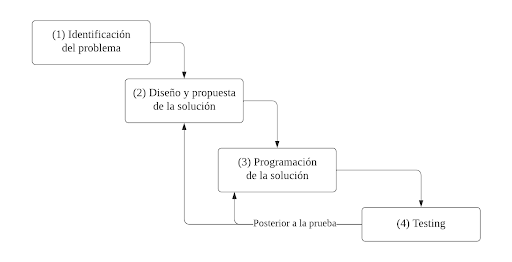
\includegraphics[scale=.9]{imagenes/ProcesoDeDisenoDiagrama.png}
	\caption{Proceso de desarrollo iterativo llevado a cabo para crear IGACSE.}
	\label{ProcesoDeDiseno}
\end{figure}


\subsection{Identificación del problema}

Previo a las decisiones de diseño que dan origen a las mecánicas de juego, Según Rogers en su libro sobre diseño interactivo \cite{Rogers2002InteractionDesign}, es crucial identificar el problema que se busca resolver, qué usuarios se ven afectados por este problema, qué características poseen y cómo podría resolverse en base a prototipos.

El diseño del videojuego surge a partir de la identificación de un problema recurrente entre los estudiantes de computación: la dificultad para comprender completamente los algoritmos enseñados. Esta falta de comprensión, a menudo no reconocida por los propios estudiantes, se manifiesta en la incapacidad para reproducir los pasos de los algoritmos de manera precisa, especialmente en situaciones como exámenes o tareas donde se requiere seguir instrucciones al detalle.

Se parte del supuesto de que, en muchas ocasiones, los estudiantes creen entender cómo funciona cierto código o algoritmo, pero no lo aplican paso a paso con papel y lápiz. Al asignarles como ejercicio realizar el procedimiento siguiendo cada instrucción rigurosamente, los estudiantes no lo llevan a cabo o lo hacen de forma incorrecta sin percatarse de sus errores. Un estudio de Zingaro et al. \cite{IdentifyingStudentDifficultiesDataStructures} corrobora esta situación, indicando que los estudiantes a menudo creen entender los contenidos, pero presentan conceptos erróneos sin ser conscientes de ellos.

El trabajo de Zingaro et al. \cite{IdentifyingStudentDifficultiesDataStructures} ejemplifica estos malentendidos, mencionando errores al comprender estructuras de datos como los heaps y las formas en que pueden representarse o construirse.

A un nivel más particular, en la Universidad de Chile, tanto históricamente como hasta la actualidad, para obtener la licenciatura en computación se exige aprobar dos años de cursos de plan común. Durante este período, los estudiantes practican una técnica conocida como ``pauteo'', que implica estudiar y revisar pautas de pruebas y tareas de semestres anteriores para prepararse para los exámenes. Esta práctica lleva a los estudiantes a centrarse en la revisión de los procesos para responder preguntas, sin necesariamente realizar los ejercicios o repetir los pasos de manera detallada, lo que resulta en un aprendizaje superficial de los contenidos.

La práctica del ``pauteo'' resulta especialmente perjudicial en el área de grafos y sus algoritmos. Si bien los estudiantes pueden captar los conceptos básicos o memorizar las ideas generales explicadas en clase, a menudo no logran reproducir paso a paso algoritmos como BFS y DFS, lo que limita su comprensión profunda de la materia.

Para abordar este problema, se propone el desarrollo y evaluación de una herramienta que, mediante una interfaz visual interactiva, proporcione una experiencia lúdica y atractiva para el usuario, facilitando la comprensión y reproducción paso a paso de los algoritmos.

Cabe señalar que, para enseñar los conceptos relacionados con programación, el escenario ideal consta de usuarios que tengan nociones de programación, pero que carezcan de años de experiencia, lo suficiente para que no puedan comprender un algoritmo a cabalidad con solo ver el código. Por lo mismo, se propone utilizar un modelo similar a los depuradores o debuggers, donde se puede ver el estado de las variables en cada paso, así como la instrucción por ejecutarse y el resultado que conlleva.


\subsection{Diseño y propuesta de la solución}

La fase inicial del diseño involucró la creación de diversos bocetos de interfaz, basándose en ciertos referentes mencionados en este trabajo. Se presentó semanalmente el trabajo de tesis al curso ``CC7970 - Trabajo de Tesis I'' compuesto por un grupo de 20 estudiantes de posgrado de ciencias de la computación. Los alumnos del curso daban sus comentarios en cada clase. Tras analizar las opciones, se seleccionó un diseño que destacaba por su claridad, atractivo y similitud con el entorno de desarrollo Visual Studio Code.

Como prerrequisitos se establecieron los siguientes aspectos: el videojuego creado debe evitar la mecanización por parte del estudiante, instándolo a revisar de manera consciente y exhaustiva cada paso relacionado con el algoritmo, y que no dé por sentado que se entiende el código y saltar a la siguiente actividad; como punto de referencia visual, el trabajo se inspira parcialmente en el debugger (depurador) de Visual Studio Code. Esta herramienta permite visualizar los valores de las variables en cada momento, además de avanzar paso a paso a lo largo del código, facilitando la comprensión de los algoritmos de manera detallada.

Con lo anterior, se implementaron diversas versiones del juego utilizando Godot, un motor de juegos que permite agregar nuevas funcionalidades de manera rápida y flexible, manteniendo un diseño visual consistente.

Además, para validar la efectividad del juego, se realizaron pruebas con usuarios expertos. Estos experimentaron dificultades para seguir y comprender los algoritmos presentados, lo evidenció que el juego no alcanzaba su objetivo principal con personas sin experiencia previa en grafos. Ante este hallazgo, se recurrió a la asesoría directa de diseñadores de videojuegos, expertos en diseñar interfaces de usuario (UI) y de experiencia de usuario (UX).

Los diseñadores asesores sugirieron la inclusión de tutoriales que mostraran los elementos del juego de manera gradual. Adicionalmente, se propuso incorporar una narrativa de fondo que permitiera a los jugadores identificarse con el juego y comprender la utilidad práctica de los algoritmos y estructuras que estaban aprendiendo. Se enfatizó la importancia de agregar elementos de premiación y ludificación para incrementar la motivación y el compromiso de los usuarios con el juego.

Tras finalizar los tutoriales e integrar los estilos, la música y los elementos narrativos, se procede a publicar el videojuego en la plataforma Itch.io, un sitio web dedicado a la venta de videojuegos y elementos relacionados, especialmente de creadores independientes o con recursos limitados.

\subsection{Referentes}

Los referentes más importantes son aquellos videojuegos que tienen un rol educativo relacionado a la programación, como 7 Billion Humans \cite{7billionhumans} (Figura \ref{7BillionHumans}) y CodeCombat \cite{CodeCombat} (Figura \ref{CodeCombat}).

\begin{figure}[h]
	\centering
	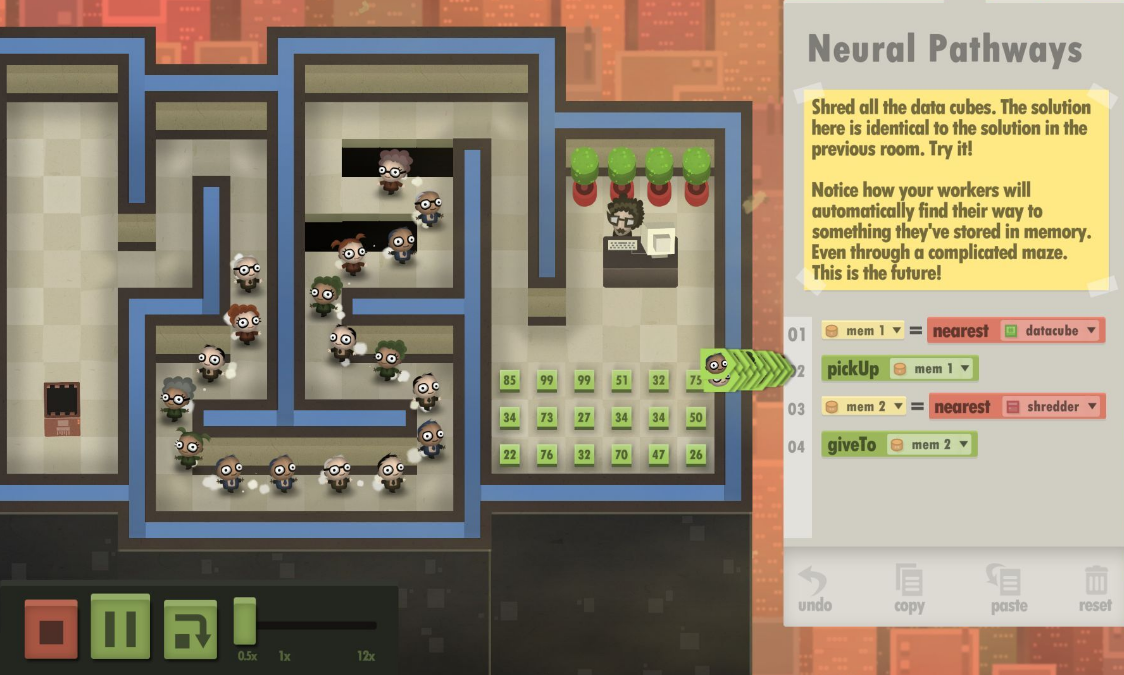
\includegraphics[scale=0.3]{imagenes/7BillionHumans.png}
	\caption{Videojuego 7 Billion Humans}
	\label{7BillionHumans}
\end{figure}

\begin{figure}[!h]
	\centering
	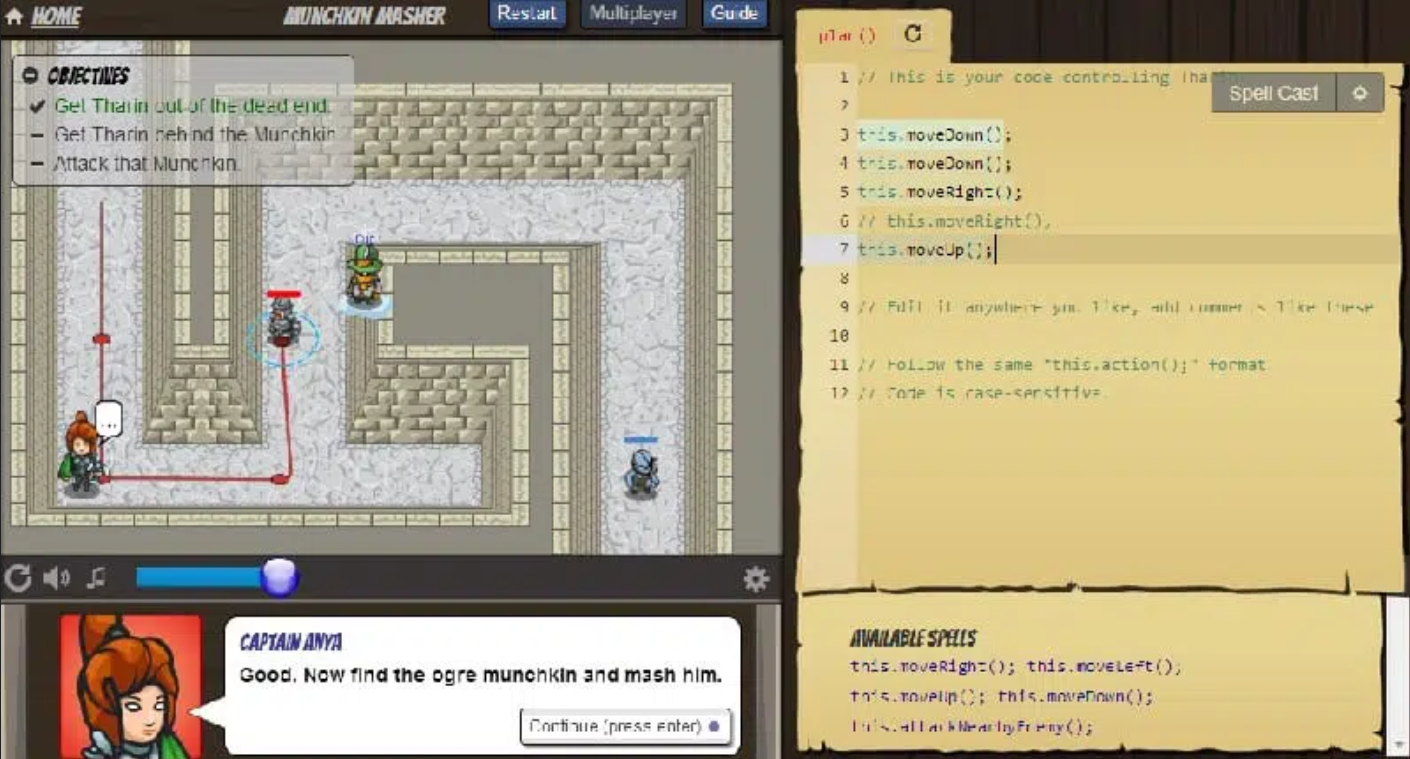
\includegraphics[scale=0.3]{imagenes/CodeCombat.png}
	\caption{Videojuego CodeCombat}
	\label{CodeCombat}
\end{figure}

Estos juegos presentan ventanas de texto prominentes en la interfaz principal, que ocupan al menos el 20\% de la pantalla. Además, incluyen diálogos que contribuyen a una narrativa continua, situados en la parte inferior de la ventana gráfica al inicio y al final de cada nivel. En ambos casos, la interfaz de código se encuentra en el lado derecho, lo que permite al usuario observar cómo la ejecución de las instrucciones afecta al juego paso a paso.

A partir de este análisis, se concluye que es requisito del juego mostrar la ejecución del código instrucción por instrucción.

Adicionalmente, se revisaron canales de YouTube educativos como 3Blue1Brown \cite{3Blue1BrownYT} (Ver figura \ref{3B1BYTChannelThumbnail}), donde el propietario del canal, Grant Sanderson, habla repetidamente sobre cómo las visualizaciones ayudan a comprender la abstracción matemática subyacente. 

\begin{figure}[!h]
	\centering
	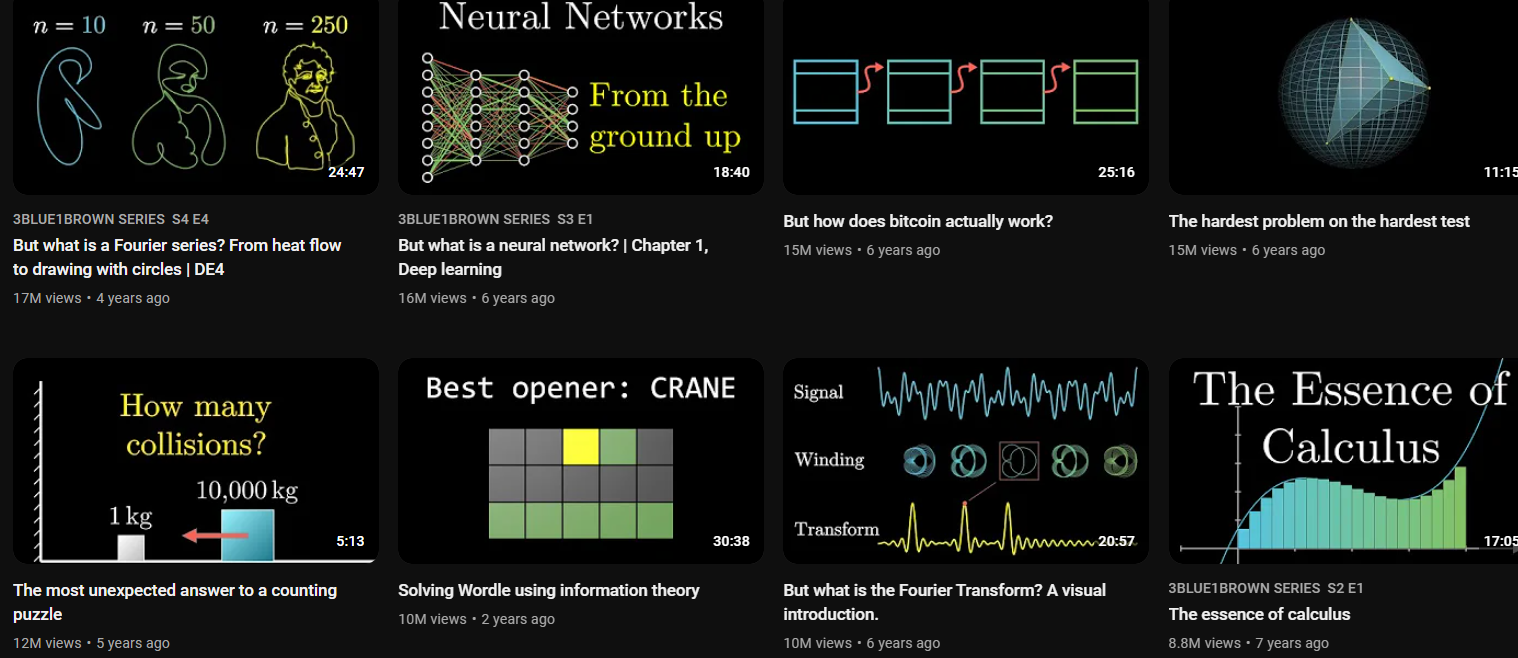
\includegraphics[scale=0.5]{imagenes/3B1BChannel.png}
	\caption{Thumbnail del canal de Youtube 3B1B de Grant Sanderson. Aquí se muestra cómo explica conceptos abstractos con visualizaciones y animaciones \cite{3Blue1BrownYT}.}
	\label{3B1BYTChannelThumbnail}
\end{figure}


\subsection{Diseño de la interfaz de usuario}


La interfaz de usuario está basada principalmente en el depurador (debugger) de Visual Studio Code \cite{vscode} (Ver figura \ref{VScodeDebugger}). Se observa aquí que la instrucción actual está destacada a través de un puntero y un énfasis con color. Además, las variables locales muestran su valor en un formato “nombre: valor”. El usuario puede avanzar paso a paso en el código.

\begin{figure}[h]
	\centering
	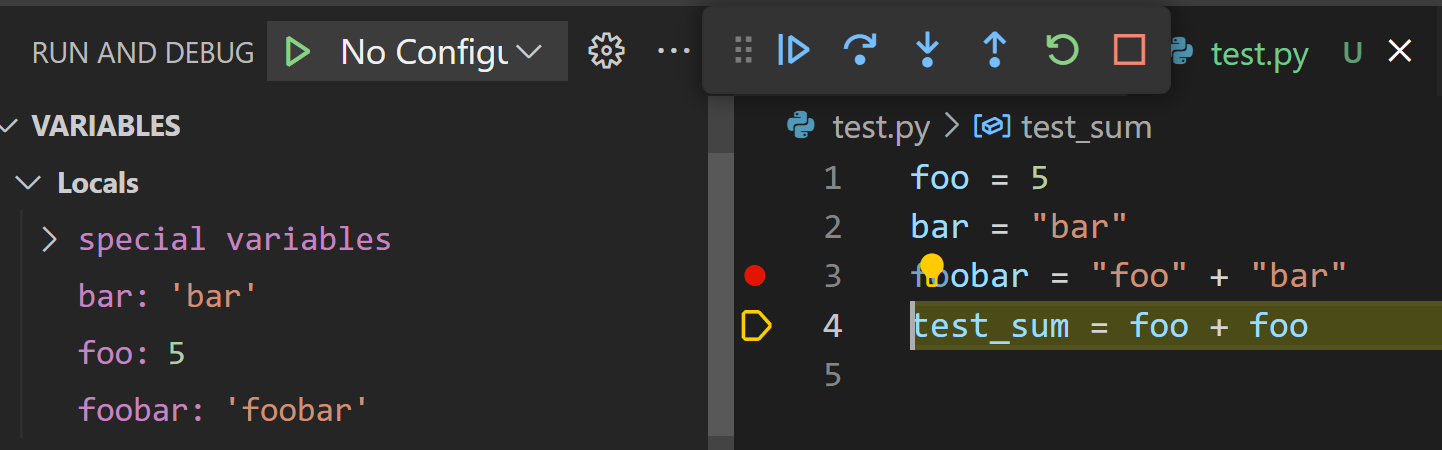
\includegraphics[scale=0.5]{imagenes/VScodeDebugger.png}
	\caption{Visual Studio Code Debugger.}
	\label{VScodeDebugger}
\end{figure}

Hay otros juegos cuya interfaz sirvió de inspiración para la realización del juego final, como 7 Billion Humans \cite{7billionhumans}, donde el código se ve a la derecha de la pantalla. La porción que contiene los elementos y eventos del juego está al lado izquierdo. Lo que ocurre en la interfaz de la derecha afecta al mundo virtual, tal como en la aplicación IGACSE.

Otro videojuego con una interfaz similar es CodeCombat \cite{CodeCombat}. Aquí el código también está a la derecha, mientras que abajo se ven diálogos y elementos seleccionables. En el caso de IGACSE, los diálogos también se muestran abajo, así como las variables actuales y la seleccionada. Además, el menú del juego se accede en la esquina superior izquierda (Ver figura \ref{CodeCombat}).

En resumen, se observa que existen videojuegos educativos que dedican una gran parte de su interfaz a mostrar código al lado derecho, como CodeCombat y 7 Billion Humans, además de mostrar el estado del juego en la parte inferior. En el caso de IGACSE, se hizo lo mismo como se puede ver en la figura \ref{InterfazBFS}.

\begin{figure}[h]
	\centering
	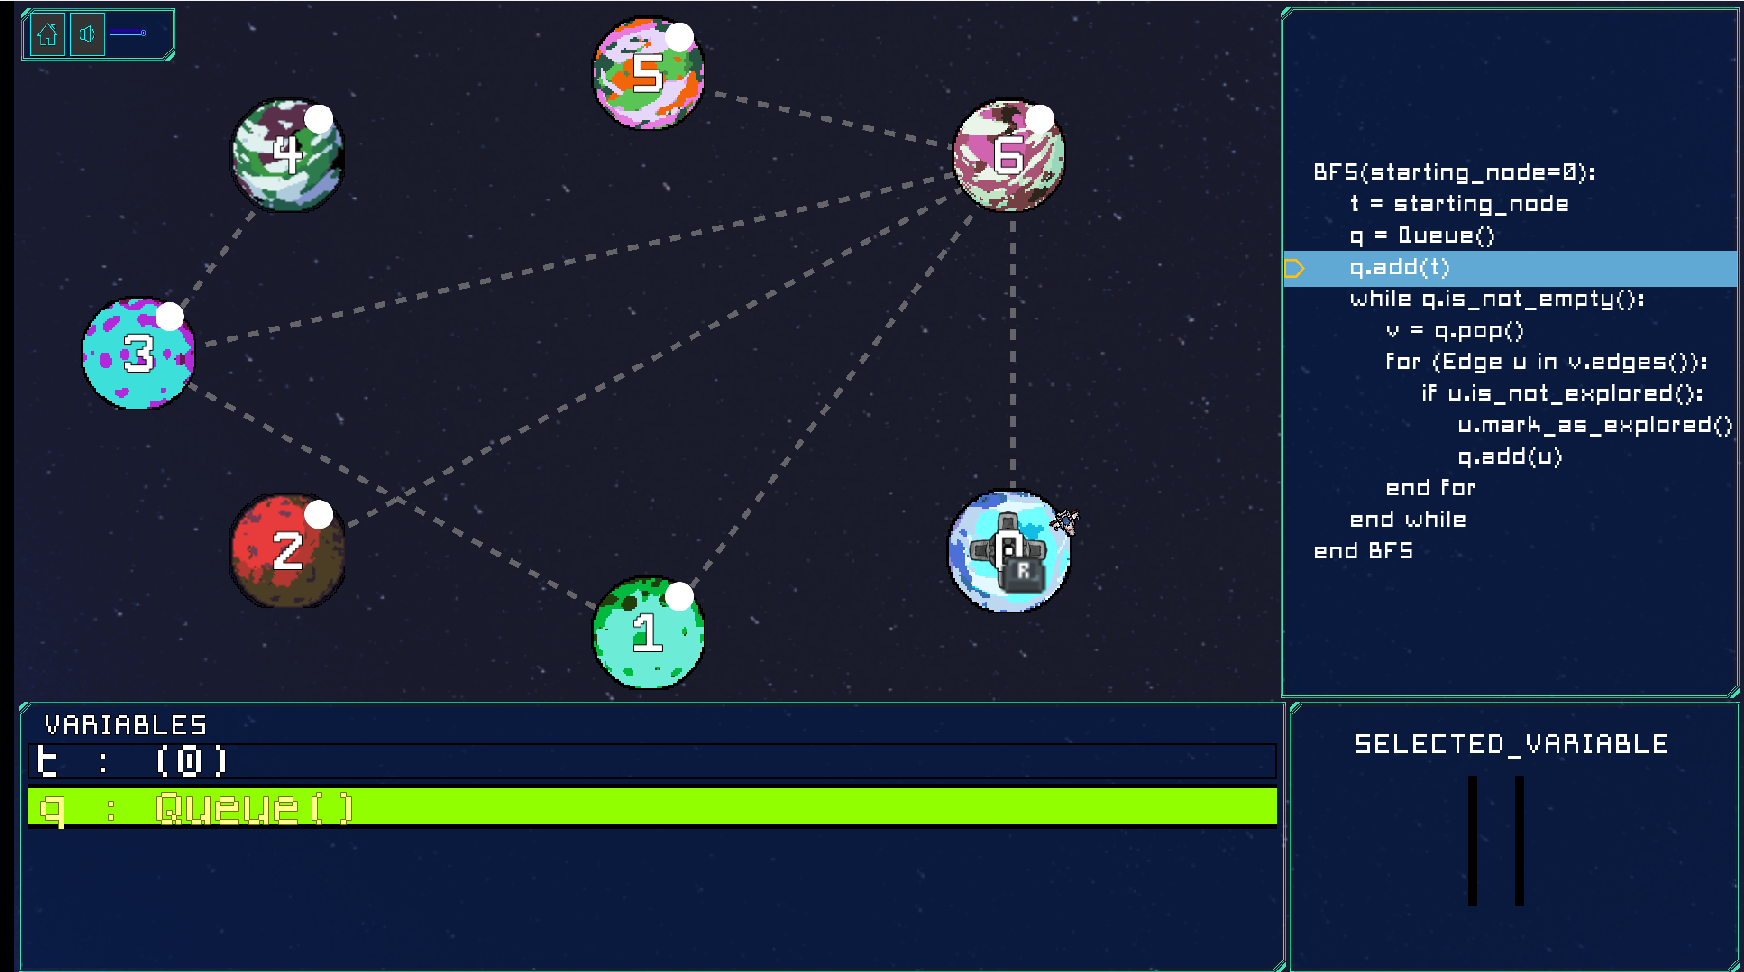
\includegraphics[scale=0.5]{imagenes/InterfazBFS.png}
	\caption{Interfaz del nivel BFS de IGACSE. A la derecha se observa el código del algoritmo, con un especial énfasis en la línea de código actual. Por otra parte, en el lado inferior de la pantalla se ve el estado de las variables.}
	\label{InterfazBFS}
\end{figure}


\subsection{Diseño de efectos de sonido y música}

Los juegos retro comúnmente emplean bucles de música de 8 a 16 bits. Ejemplos notables incluyen Golden Sun \cite{Wiki_Golden_Sun}, ProtoCorgi \cite{ProtoCorgi}, Pokemon Emerald \cite{PokemonEmerald}, Space Invaders \cite{SpaceInvaders}, y Final Fantasy IV \cite{FinalFantasyIV}.

En juegos como Pokemon \cite{PokemonEmerald} y Golden Sun \cite{Wiki_Golden_Sun}, cada vez que se hace click en algún botón y se gatilla un evento, se emite un sonido de confirmación, como cuando el jugador selecciona un ataque. El objetivo es confirmarle al usuario que se está ejecutando correctamente una acción. IGACSE sigue una estrategia similar, utilizando sonidos agudos de confirmación al hacer clic en planetas, caminos o al presionar teclas correctamente (espacio o R). Estos sonidos nítidos cumplen la función de validar la ejecución exitosa de una acción sin distraer al jugador.

En contraste, los sonidos de error en IGACSE emplean tonos graves con desvanecimiento, generando una sensación de vibración (ver figura \ref{EspectroOndasSonidoError}). Estos sonidos más intensos se activan cuando el jugador comete errores, como hacer clic en un planeta incorrecto o un camino equivocado, presionar una tecla antes de completar una instrucción, o responder incorrectamente a preguntas del tipo Sí/No. La intención es que el jugador reconozca inmediatamente los errores y tome medidas correctivas.

\begin{figure}[h]
	\centering
	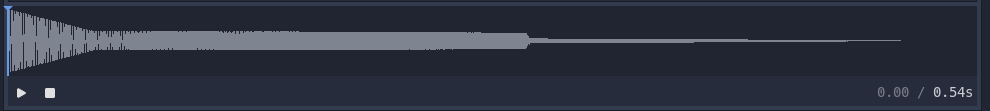
\includegraphics[width=0.9\textwidth]{imagenes/EspectroOndasConfirmacion.png}
	\caption{Espectro de Ondas del sonido de Confirmación de IGACSE}
	\label{EspectroOndasSonidoConfirmacion}
\end{figure}

\begin{figure}[h]
	\centering
	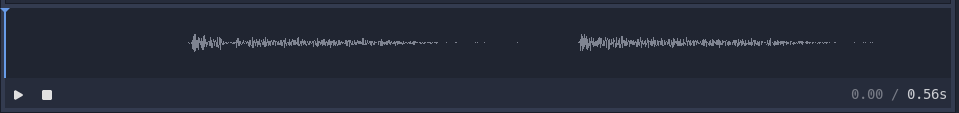
\includegraphics[width=0.9\textwidth]{imagenes/EspectroOndasError.png}
	\caption{Espectro de Ondas del sonido de Error de IGACSE}
	\label{EspectroOndasSonidoError}
\end{figure}


\subsection{Diseño de mecánicas de juego}

La condición de victoria en cada nivel implica completar todas las instrucciones proporcionadas por el algoritmo. En los niveles de BFS y DFS, esto implica visitar todos los nodos del grafo. El puntero de instrucciones señala la tarea actual, y el jugador debe ejecutar correctamente lo indicado en la instrucción, ya sea haciendo clic, respondiendo una pregunta, o agregando un nodo a una estructura de datos (Ver figura \ref{BFSExplicacion1}). Algunas instrucciones, especialmente aquellas que contienen la palabra clave for, no requieren acción por parte del jugador. Una vez que se han ejecutado correctamente los pasos requeridos, la instrucción cambiará de color y el cursor se transformará en un ticket (Ver figura \ref{BFSExplicacion2}).

\begin{figure}[h]
	\centering
	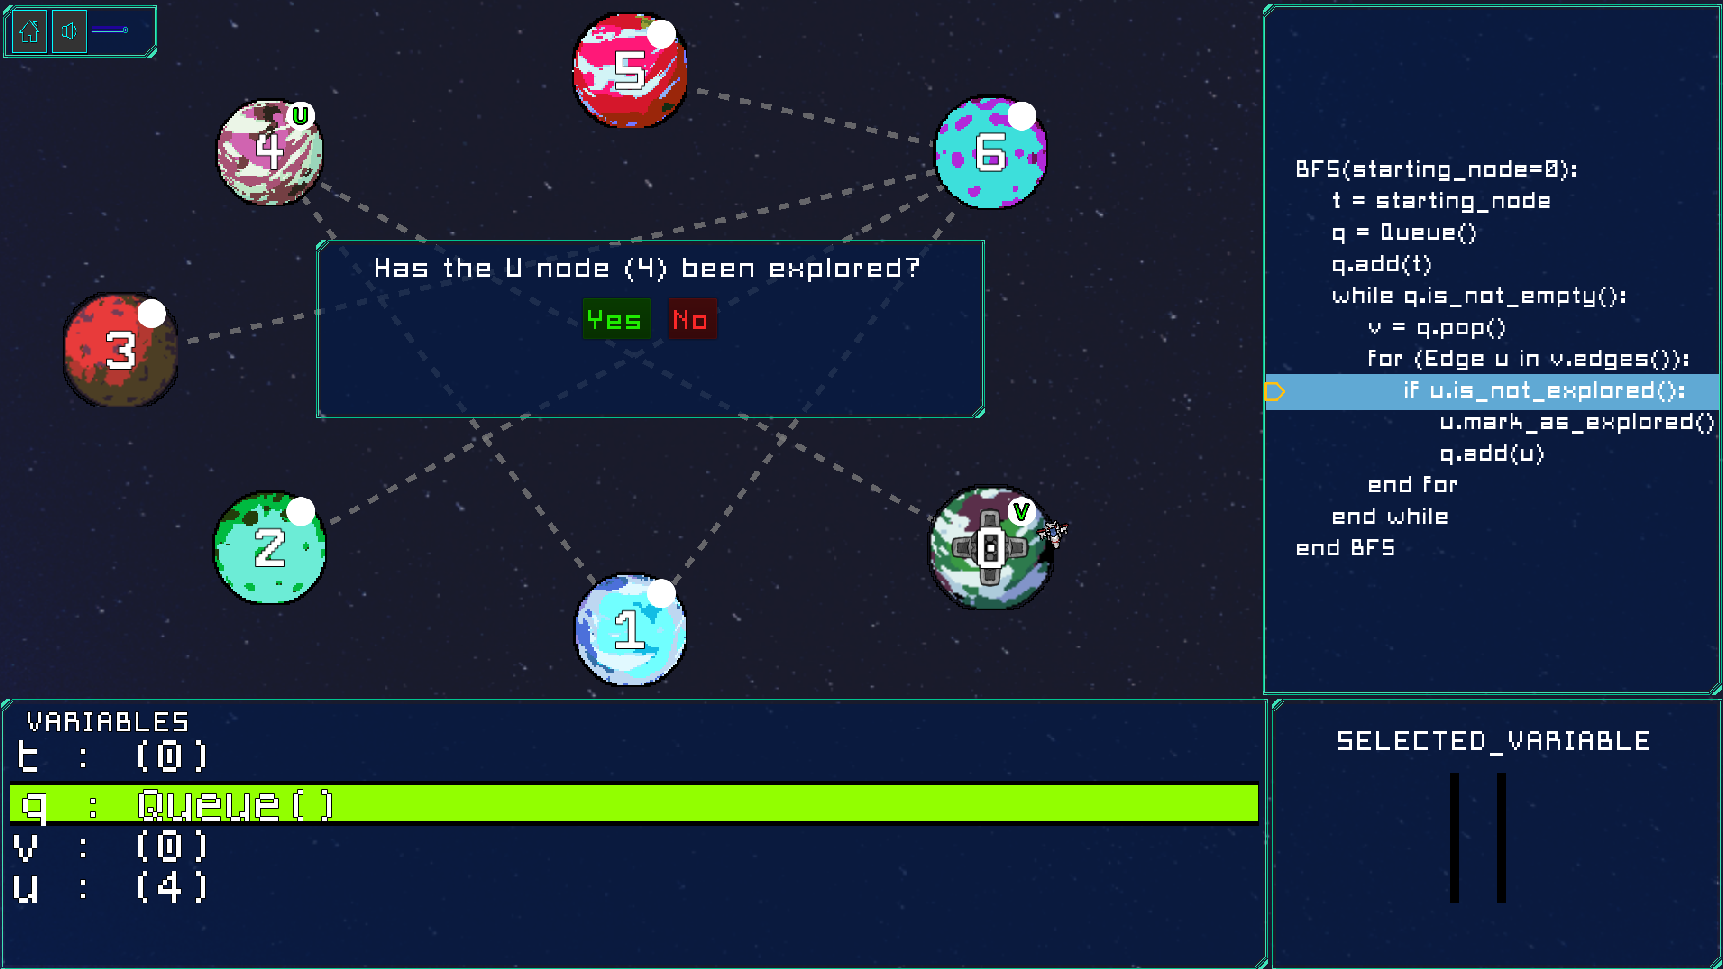
\includegraphics[width=0.9\textwidth]{imagenes/BFS_Explicacion1.png}
	\caption{El jugador está en la instrucción \textit{if u.is\_not\_explored():} El usuario debe responder correctamente sí o no. En caso de respuesta correcta, la instrucción se desbloqueará y podrá pasar a la siguiente instrucción.}
	\label{BFSExplicacion1}
\end{figure}

\begin{figure}[h]
	\centering
	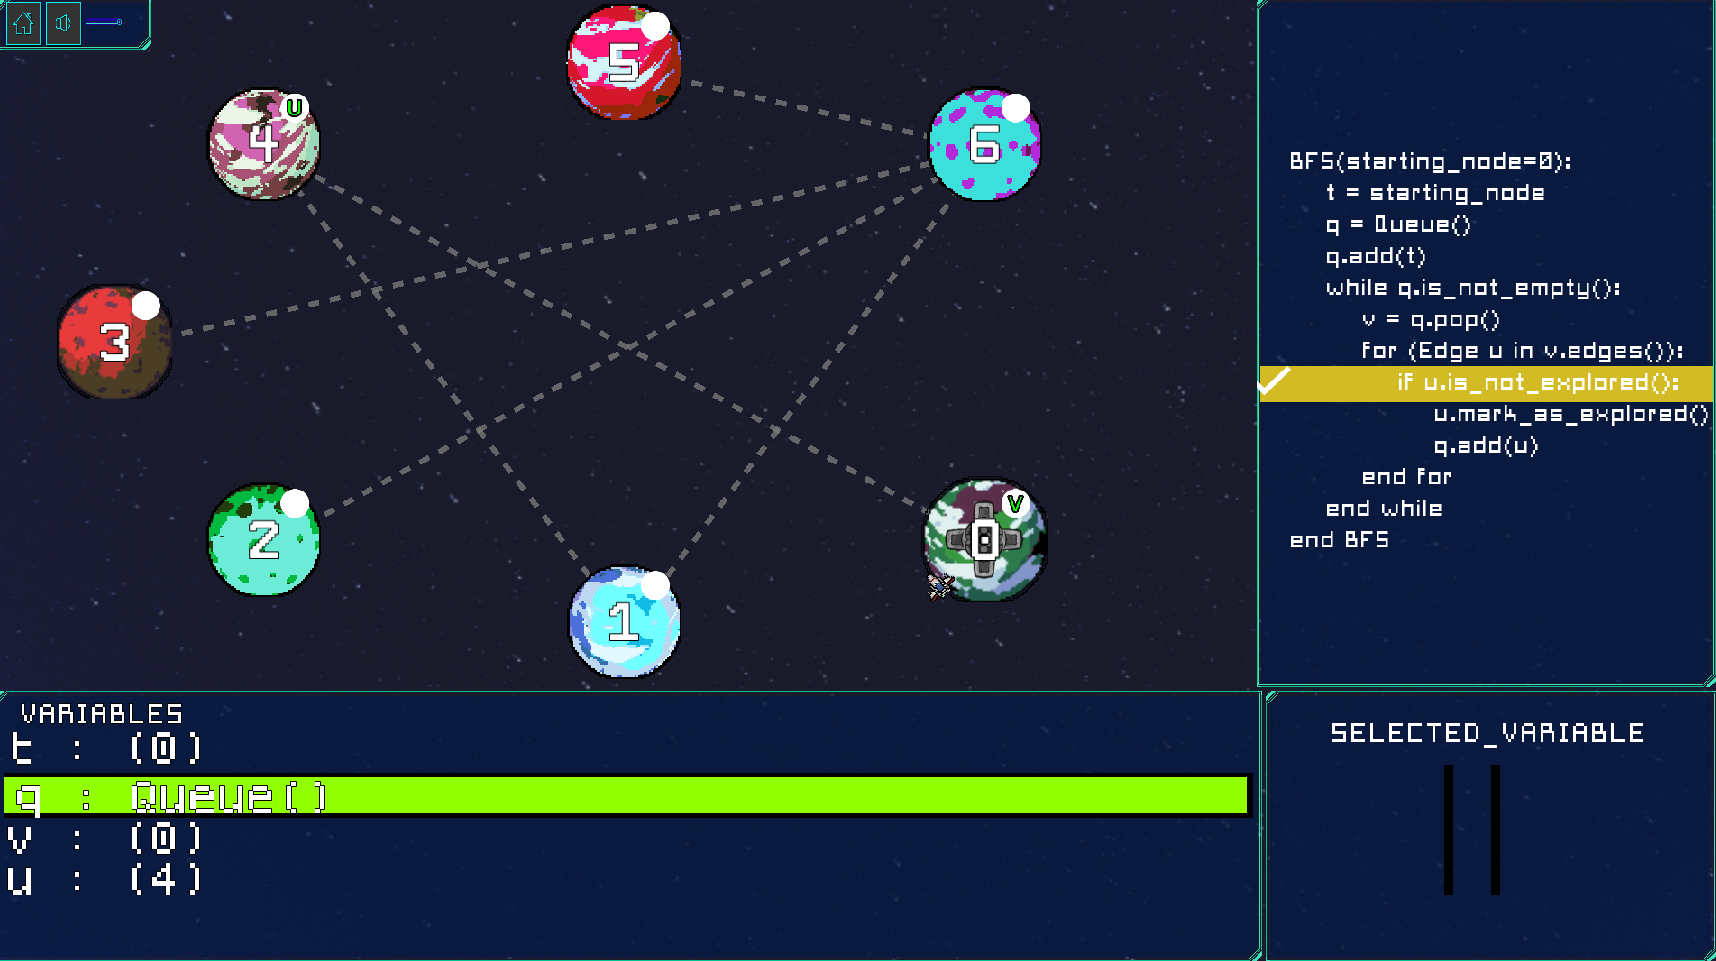
\includegraphics[width=0.9\textwidth]{imagenes/BFS_Explicacion2.png}
	\caption{El jugador está en la instrucción \textit{if u.is\_not\_explored():} después de responder correctamente, la instrucción cambia de color. Ahora se puede pasar a la siguiente instrucción.}
	\label{BFSExplicacion2}
\end{figure}


Para avanzar en las instrucciones, el jugador debe presionar la tecla espacio. Si esta se presiona sin completar la instrucción, se activará un sonido de error y el color de la instrucción parpadeará entre rojo y amarillo durante un segundo. Presionar la tecla espacio después de completar la instrucción generará un sonido de confirmación y avanzar a la siguiente instrucción. Si se presiona la tecla espacio cuando no hay más instrucciones, se emitirá un sonido de victoria, permitiendo al jugador pasar al siguiente nivel o visualizar los créditos según corresponda. Este proceso se resume en el diagrama \ref{FlujoDeMecanicasDeNivel}.

\begin{figure}[h]
	\centering
	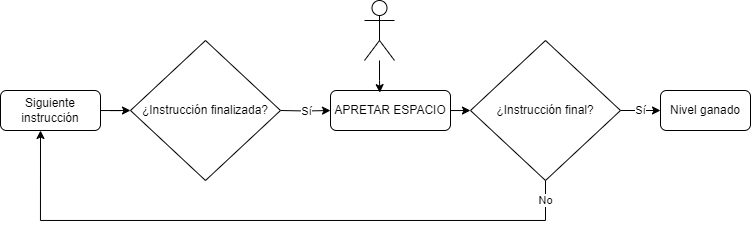
\includegraphics[width=0.7\textwidth]{imagenes/FlujoDeMecanicasDeNivel.drawio.png}
	\caption{Flujo de mecánicas de un nivel jugable. El jugador debe seguir las instrucciones paso a paso. Fuente: Elaboración Propia.}
	\label{FlujoDeMecanicasDeNivel}
\end{figure}



\section{Descripción de IGACSE}

\subsection{Flujo de juego}

El juego comienza presentando el menú principal, donde se pueden elegir dos opciones: el modo historia o los niveles jugables. Si se opta por el modo historia, se accede a los tutoriales. Una vez completados los tutoriales, se desbloquea el primer nivel jugable, que corresponde al algoritmo DFS. Por otro lado, si se eligen los niveles jugables desde el menú principal, se muestra una lista de niveles disponibles, entre los que se encuentra el algoritmo BFS y DFS. Al completar cada uno de estos niveles, se muestran los créditos del juego (Ver figura \ref{FlujoDeJuego}).

El videojuego se divide en distintas escenas, que incluyen el menú principal, los tutoriales y los niveles jugables. En el menú principal, los jugadores pueden seleccionar el nivel que desean jugar o acceder al modo historia. Los tutoriales están diseñados para introducir conceptos básicos de grafos sin mencionar explícitamente el término "grafo", con el objetivo de no interrumpir la narrativa. Además de los conceptos teóricos, los tutoriales enseñan habilidades de juego, como explorar o seleccionar nodos, ejecutar instrucciones de código y responder preguntas de tipo Sí/No relacionadas con las estructuras de control, como las instrucciones condicionales (if).

\begin{figure}[h]
	\centering
	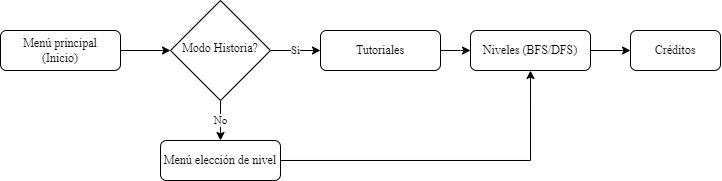
\includegraphics[scale=0.15]{imagenes/FlujoDeJuego.png}
	\caption{Flujo de juego de IGACSE. Fuente: Elaboración propia.}
	\label{FlujoDeJuego}
\end{figure}


Finalmente, el juego presenta los niveles, que corresponden a los algoritmos que se desean enseñar: BFS (Breadth First Search) y DFS (Depth First Search). En estos escenarios, no hay avance en la narrativa ni guía para el usuario. Una vez que se completan, se muestran los créditos del juego.

El juego se enfoca en la exploración de planetas a través de rutas, utilizando una metáfora de grafos donde los planetas representan nodos y los caminos entre ellos son aristas. El objetivo es rescatar pandas rojos dispersos en los planetas. Para lograrlo, es necesario explorar todos los nodos en una galaxia, que corresponde a un nivel del juego. En cada nivel, se enseña un algoritmo diferente. Se utiliza una narrativa ficticia para ayudar en la comprensión de los conceptos de grafos.

Durante el juego, se proporcionan instrucciones en el lado derecho de la pantalla, a medida que el jugador avanza presionando la tecla espacio. Cada vez que se avanza en las instrucciones, se desencadenan efectos y animaciones que muestran visualmente lo que está sucediendo en el código. Estas animaciones se reflejan en la ventana de juego, donde se destacan los planetas, los caminos o las naves que se desplazan entre planetas.

Siguiendo las instrucciones paso a paso, el jugador repite el algoritmo, lo que le permite entender cómo funciona y cuál es su finalidad. Las acciones del jugador pueden ir acompañadas de sonidos de recompensa, que indican el avance a la siguiente instrucción. En caso de cometer un error, se notifica al jugador mediante una animación visual y un sonido. En ciertos casos, si el jugador no sabe qué hacer, se muestra un hint visual que le indica qué tecla debe presionar o qué acción debe realizar.



\subsection{Narrativa}

Para la visualización de algoritmos como el BFS y DFS, ampliamente conocidos como algoritmos de búsqueda de rutas, se realizan representaciones que requieren del enrutamiento de redes, mapeo de ubicaciones, telecomunicaciones y la navegación \cite{surti2023NeoRoute}. Estas representaciones ayudan en la comprensión de los conceptos de grafos y establecen las bases para la narrativa ficticia que acompañará al usuario durante el desarrollo del videojuego.

Es por ello que el juego se enfoca en su utilidad más común, utilizando como metáfora narrativa la exploración de planetas a través de rutas, donde los planetas representan nodos y los caminos entre ellos son aristas. El objetivo final del juego es rescatar pandas rojos dispersos en los planetas. Para lograrlo, es necesario explorar todos los nodos en una galaxia, que corresponde a un nivel del juego. En cada nivel, se enseña un algoritmo diferente.

La narrativa se desenvuelve en el espacio exterior, donde una nave entabla un diálogo con una estación llamada DCC. La misión de la nave es rescatar pandas rojos dispersos en los planetas de la galaxia. Inicialmente, el piloto señala que los niveles de combustible son bajos, y la estación sugiere continuar con las siguientes galaxias, evitando el uso del piloto automático debido al alto costo y consumo de combustible de las redes neuronales. Para optimizar recursos, la nave deberá seguir instrucciones manuales para completar la misión. Con cada galaxia visitada, el piloto rescata y encuentra otros pandas rojos. Se premia al jugador para que continúe con los siguientes niveles y complete el juego.

Es relevante destacar que la estación se llama DCC para aumentar el sentido de identificación con el jugador, ya que DCC son las siglas del Departamento de Ciencias de la Computación. Además, el panda rojo es la mascota oficial del Centro de Alumnos del Departamento de Ciencias de la Computación (CADCC). Durante las actividades de bienvenida a los nuevos estudiantes, se muestran afiches con esta mascota, por lo que se busca que el usuario se sienta identificado con el juego.
 

\subsection{Menú principal}

En el menú principal, se puede seleccionar el idioma presionando el botón en la esquina superior izquierda de la figura \ref{MenuPrincipal}. Los idiomas disponibles son inglés y español. Además, ofrece las opciones para jugar en el modo historia o los niveles jugables.


\begin{figure}[h]
	\centering
	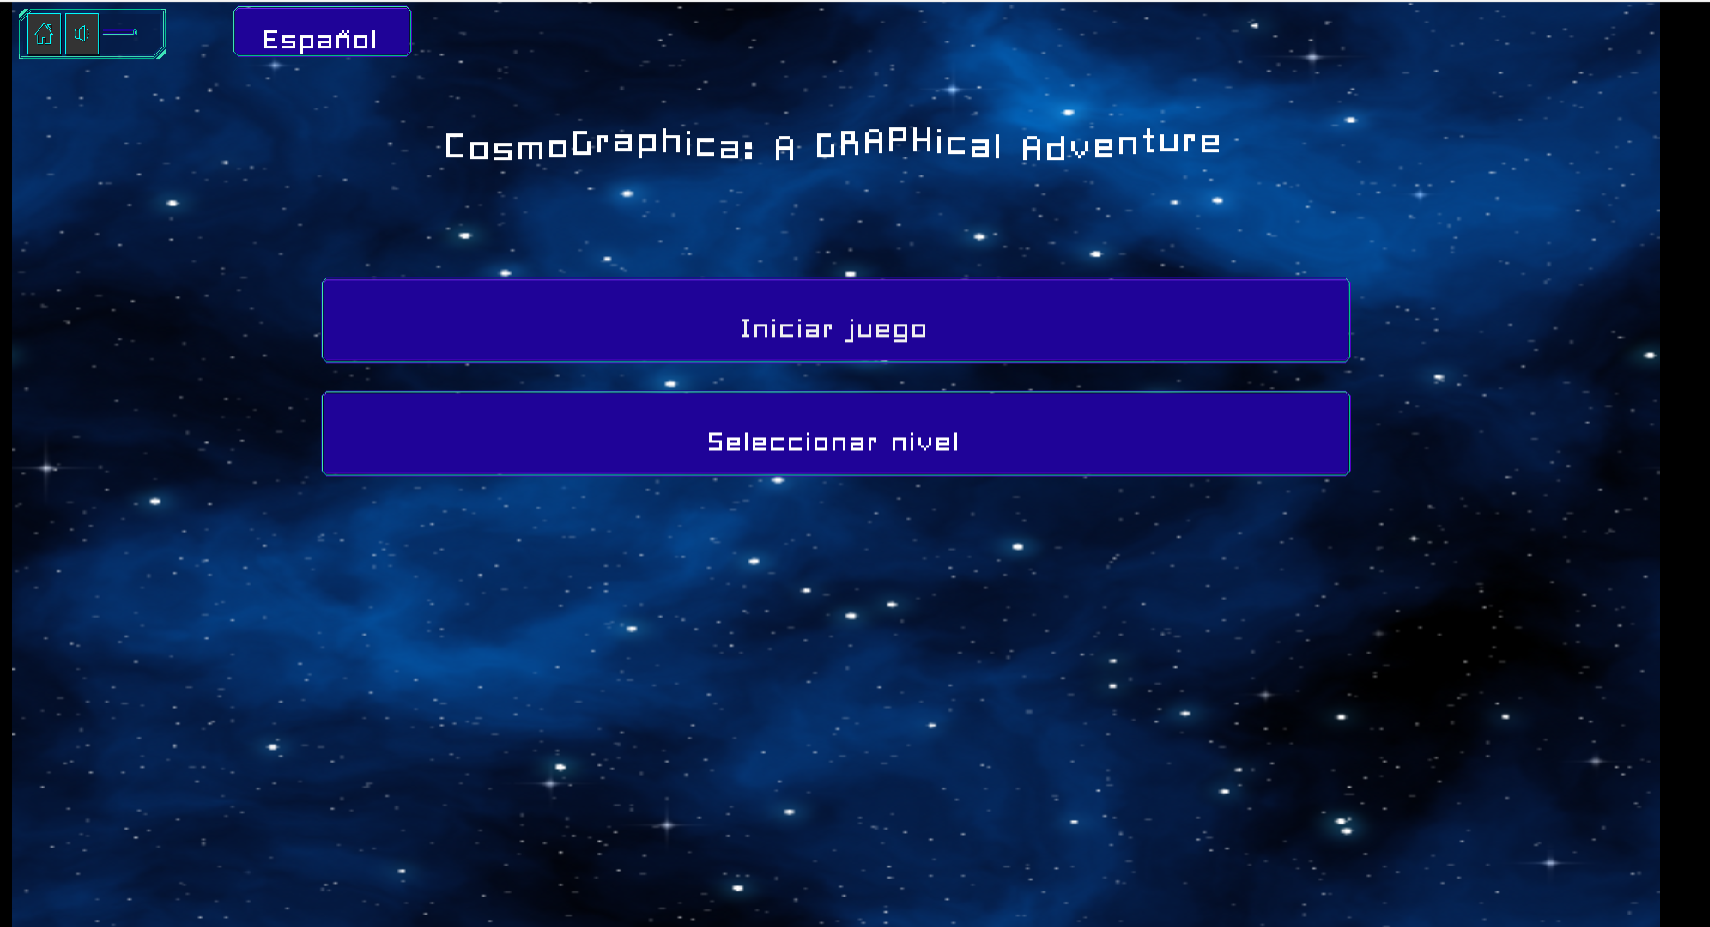
\includegraphics[scale=0.33]{imagenes/MainMenu.png}
	\caption{Menú principal de IGACSE, que se muestra al iniciar el juego.}
	\label{MenuPrincipal}
\end{figure}


\subsection{Tutoriales}

Los tutoriales persiguen dos propósitos: familiarizar al jugador con las mecánicas básicas que se emplearán a lo largo del juego y sumergirlo en la trama narrativa. Las mecánicas se introducen a través de una combinación de elementos que incluyen texto descriptivo y pistas visuales, tales como la representación de un ratón realizando un clic izquierdo o la indicación de una tecla, como la "R", siendo presionada sobre un planeta. La trama está diseñada para ejemplificar la aplicación de conceptos relacionados con los grafos sin entrar en detalles explícitos sobre el contenido que se está enseñando. Es importante destacar que cada nivel y tutorial son concebidos como elementos repetibles, lo que permite al jugador revisarlos en caso de no comprender algún aspecto específico.

Se pueden ver imágenes y explicaciones de cada tutorial en el Anexo sobre tutoriales \hyperref[AnexoHTutoriales]{anexo H}.

\subsection{Niveles}

Los niveles presentados son BFS y DFS, que enseñan esos algoritmos. Los planetas y sus conexiones son aleatorias, con la restricción de que el grafo formado es siempre conexo, es decir, todos sus nodos tienen al menos un camino hacia el resto de los otros nodos.

Se crearon 4 niveles para el juego, incluyendo los algoritmos BFS, DFS, Kruskal y Prim. Sin embargo, estos últimos no fueron incluidos en la versión final del juego, pues el diseño y la experiencia de usuario eran distintos por requerir otro tipo de acciones, como ordenar arcos y operar con conjuntos, obteniendo uniones e intersecciones. Además, el tiempo de la prueba de usuario era aproximadamente de 45 minutos, por lo que se prefirió no incluirlo en la prueba dado que no se contaba con el tiempo suficiente para probarlos.

Se espera que en posibles trabajos futuros se agreguen estos niveles, incluyendo más desafíos y estudios de usabilidad respecto a qué mecánicas podrían generarse para ordenar los arcos de un grafo por orden de pesos, o cómo operar con conjuntos. El código de estos niveles se encuentra disponible en el repositorio de GitHub \cite{GithubRepo}.


\section{Arquitectura de software}

Antes de abordar la arquitectura específica del programa, es crucial comprender cómo se estructuran los programas en Godot. Esta comprensión sirve como base para justificar las decisiones de diseño adoptadas durante el desarrollo de la aplicación.

\subsection{Arquitectura de una aplicación en Godot}

Una aplicación en Godot se construye en base a escenas. Una escena es un conjunto de objetos instanciados al mismo tiempo. Un programa creado en este motor se compone de escenas, que suelen ser los niveles en un juego. Las escenas tienen un grafo de escena compuesto por uno o más nodos (Ver figura \ref{GodotArchitectureDiagram}).

\begin{figure}[h]
	\centering
	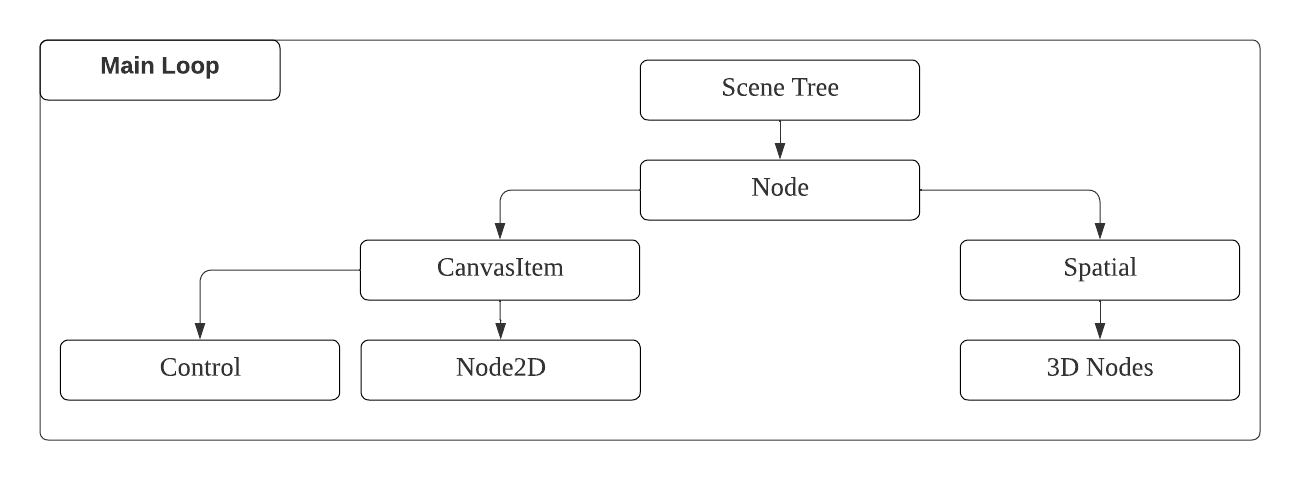
\includegraphics[scale=0.8]{Diagramas/GodotArchitectureNodes.png}
	\caption{ Estructura del Grafo de Escena de Godot. Cada elemento es un nodo, que puede ser de interfaz (control), 2D o espacial y 3D. En el caso de IGACSE, todos los elementos son de control o un Nodo 2D.}
	\label{GodotArchitectureDiagram}
\end{figure}

Los nodos en Godot son las unidades fundamentales de construcción del programa, representando diversos elementos como botones, texturas, reproductores de sonido o áreas de colisión. Para crear personajes con lógica compleja, como habilidades, movimiento y colisiones, se combinan múltiples nodos.

La estructura del grafo de escena es favorable en el desarrollo de videojuegos, ya que mover el nodo principal de un personaje implica automáticamente el movimiento de elementos asociados, como colisiones, sonidos y texturas. Esto simplifica la manipulación de elementos relacionados.

En Godot existe un ciclo principal, que itera sobre cada nodo, permitiendo que estos manifiesten sus propiedades. Por ejemplo, un nodo de imagen se puede asociar a un nodo de posición 2D. Si el nodo de posición 2D se mueve, veremos que la imagen se mueve de la misma forma. Además, se puede asociar un nodo de sonido para hacer que se emitan sonidos desde esa posición.

Esta lógica de asociación de nodos permite crear componentes rápidamente, lo que permite reutilizar código y características asociadas, como imágenes, colores y sonidos. Como Godot es de código abierto, crear nuevos nodos con sus otras propiedades resulta accesible para programadores con distintos niveles de experiencia.

Una ventaja de usar Godot frente a bibliotecas de computación gráfica como PyGame u OpenGL es la capacidad de utilizar variables exportadas. Estas variables, cuyos valores se definen desde el editor, permiten instanciar objetos de la misma clase con características distintas \cite{GodotExportVariables}.

Al trabajar a un nivel más bajo con bibliotecas como PyGame, que emplea OpenGL, requiere abordar individualmente cada aspecto de la representación de un objeto. Por ejemplo, mover un personaje implica gestionar texturas y colisiones por separado en el código, aumentando costos y complejidad en el desarrollo \cite{GodotCollisionsAndRendering}.

\begin{figure}[h]
	\centering
	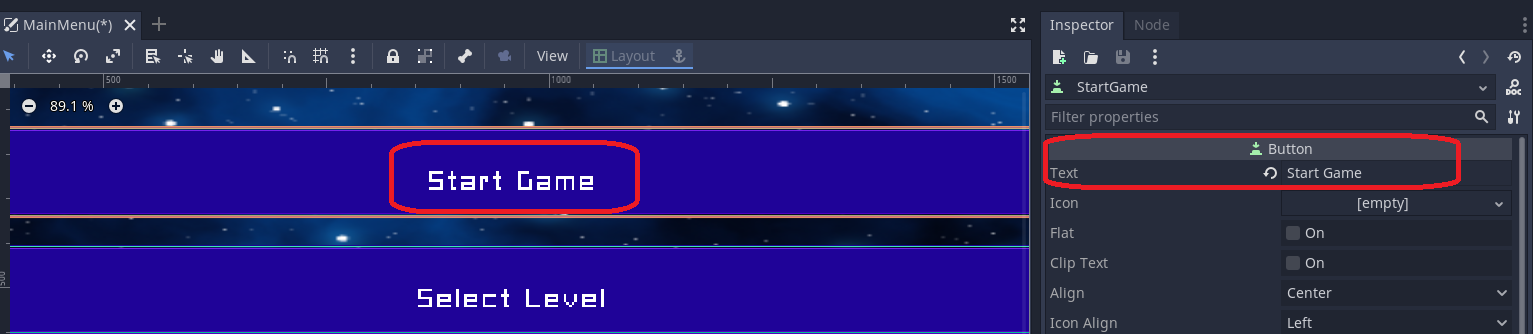
\includegraphics[scale=0.4]{imagenes/VariablesExportadas1.png}
	\caption{Variables exportadas de Godot. En este caso se muestra el menú principal al inicio del juego. Aquí, el botón destacado muestra el texto Start Game. A la derecha se muestra la variable exportada Texto. Esta se puede modificar desde el Editor de Godot.}
	\label{VariablesExportadas1}
\end{figure}

\begin{figure}[h]
	\centering
	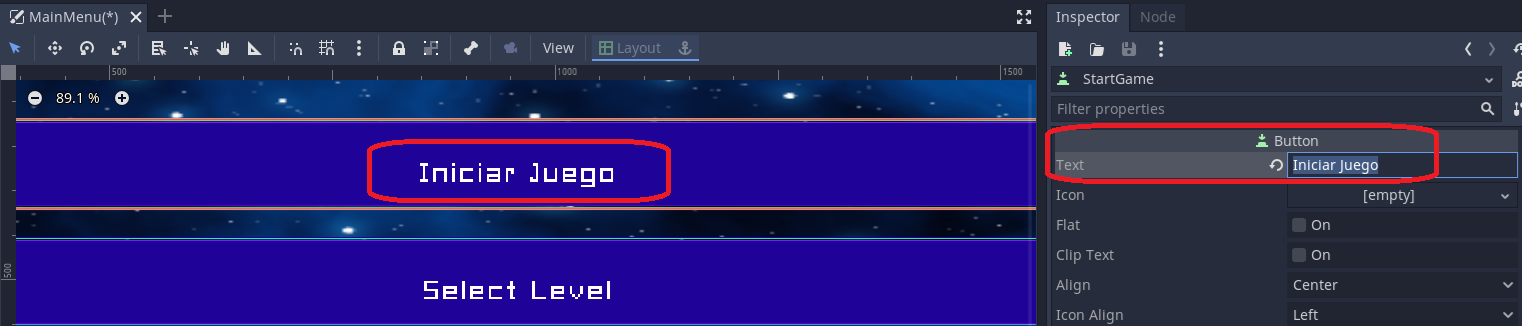
\includegraphics[scale=0.4]{imagenes/VariablesExportadas2.png}
	\caption{Siguiendo la imagen \ref{VariablesExportadas1}, el texto se modificó de Start Game a Empezar Juego. El cambio se observa de forma inmediata en la ventana, lo que permite anticipar cómo el usuario verá la escena.}
	\label{VariablesExportadas2}
\end{figure}


\subsection{Arquitectura de software de la aplicación IGACSE}

La aplicación se desarrolla en diferentes fases, las cuales abarcan tres tipos de escenas: menús, tutoriales y niveles jugables. Cada fase hace uso de módulos distintos, y cada nivel, menú o tutorial representa una escena.

Los menús se construyen principalmente mediante nodos de control, comúnmente utilizados para interfaces gráficas. En este contexto, los menús consisten principalmente en botones que ejecutan códigos específicos según su descripción, dispuestos en formato vertical o en forma de grilla (Ver figura \ref{GodotMenuInterface}).

\begin{figure}[h]
	\centering
	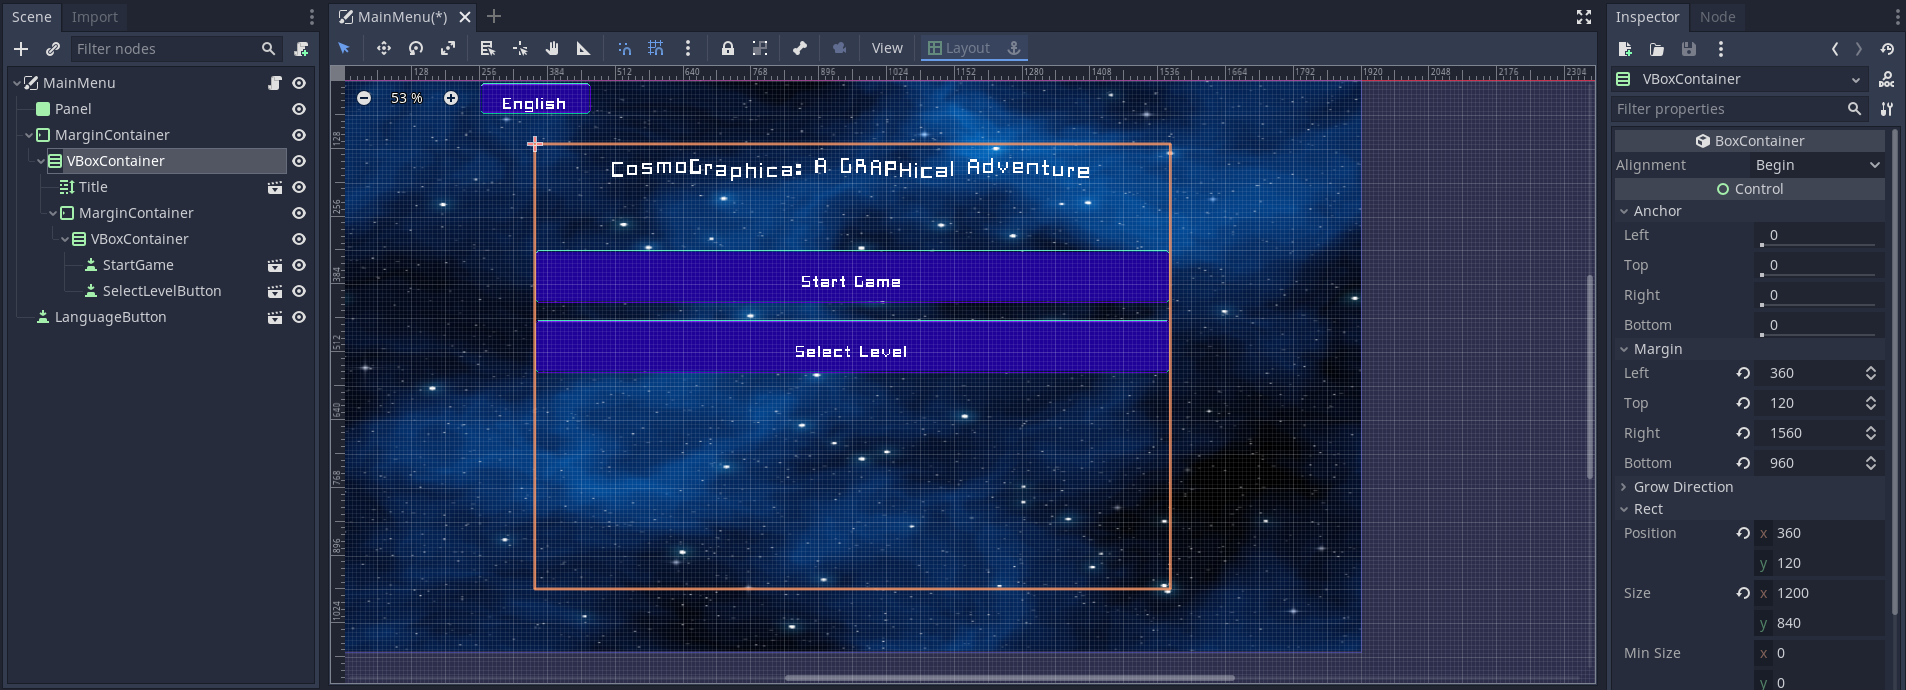
\includegraphics[width=0.9\textwidth]{imagenes/GodotInterfaceMainMenu.png}
	\caption{Interfaz de Godot describiendo la escena del menú principal de IGACSE. El juego públicamente se dio a conocer como CosmoGraphica, pero el proyecto completo se llama IGACSE.}
	\label{GodotMenuInterface}
\end{figure}


Los tutoriales presentan una lógica más compleja y se asemejan a los niveles. A diferencia de las escenas finales, los tutoriales incorporan una ventana de diálogo que busca vincular la historia del videojuego con los elementos interactivos. Además, en los tutoriales, el grafo ya está predefinido, lo que significa que los nodos y arcos ya están establecidos de antemano.

En cuanto a los niveles jugables, hay varios elementos destacables, como el código, las variables, la variable seleccionada y la ventana de juego. El grafo se representa combinando dos tipos de nodos de Godot: ``Arcos '' y ``Nodos de Grafo ''.

A modo de ejemplo, en la figura \ref{SecondTutorialGraph}, se muestra que el grafo del juego se representa en el grafo de escena en el lado izquierdo, con los nodos llamados Start, Planet2, Planet3 y StartingNode1. Los arcos se representan con los nodos Edge13, Edge1Star y Edge2S.

En la figura \ref{SecondTutorialGraph}, el arco Edge1Star está seleccionado, por lo que se muestran sus variables exportadas en el lado derecho de la pantalla. En esta sección, sale destacada el área que indica: NodeA: StartingNode y NodeB: Star. Esto genera un arco entre estos dos nodos. De esta manera, se puede crear la disposición de arcos y nodos sin necesidad de generarlos en código directamente, lo que también permite posicionar de manera predeterminada cada nodo y ver estos cambios en tiempo real.

\begin{figure}[h]
	\centering
	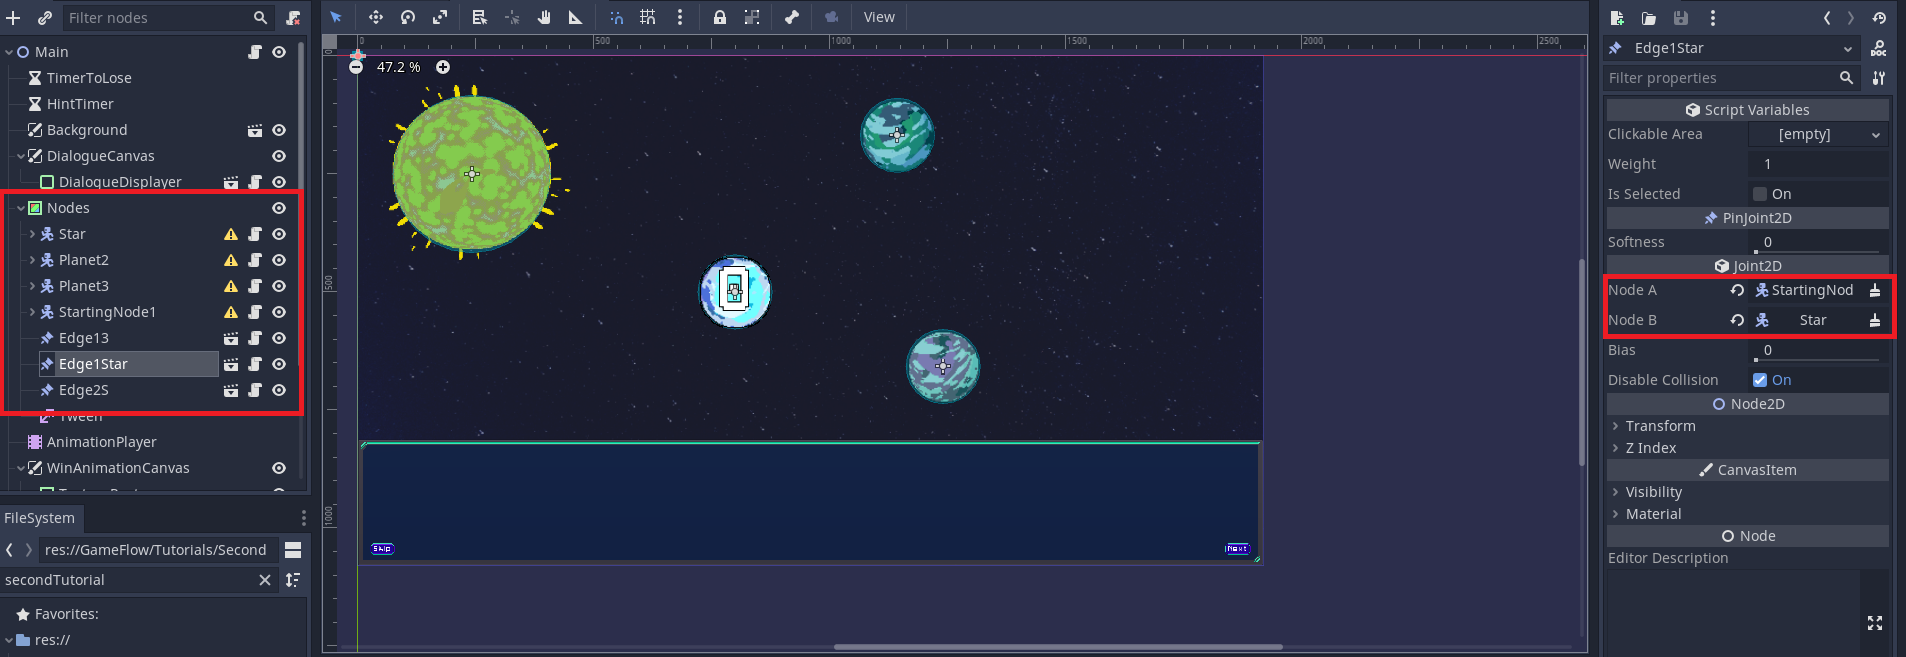
\includegraphics[width=0.9\textwidth]{imagenes/SecondTutorialGraph.png}
	\caption{Interfaz de Godot describiendo el segundo tutorial. En rojo se observa el grafo de escena con los nodos y los arcos ya predefinidos a la izquierda. En la derecha se muestra cómo se unen los arcos, indicando los dos extremos del arco a través de variables exportadas de Godot.}
	\label{SecondTutorialGraph}
\end{figure}


Respecto a la arquitectura de software presente en los niveles jugables, se observan cinco secciones en el nivel (Ver figura \ref{InterfazBFS}). Estas son: (1) El menú de opciones arriba a la izquierda; (2) La ventana de juego al centro de la pantalla; (3) El bloque de código a la derecha de la pantalla (CodeContainer); (4) Las variables existentes y sus valores en la parte inferior izquierda (DebugBlock) y, (5) La representación visual de la variable seleccionada actualmente, presente en la esquina inferior derecha de la pantalla (ADTShower).

El bloque de código que se muestra a la derecha de la pantalla durante el juego está controlado por un nodo de la clase CodeContainer. Este objeto se encarga de recibir la entrada del jugador para avanzar en el código. La clase CodeContainer posee un arreglo de objetos del tipo CodeLine llamado code lines (figura \ref{CodeLinesArchitecture}).

\begin{figure}[h]
	\centering
	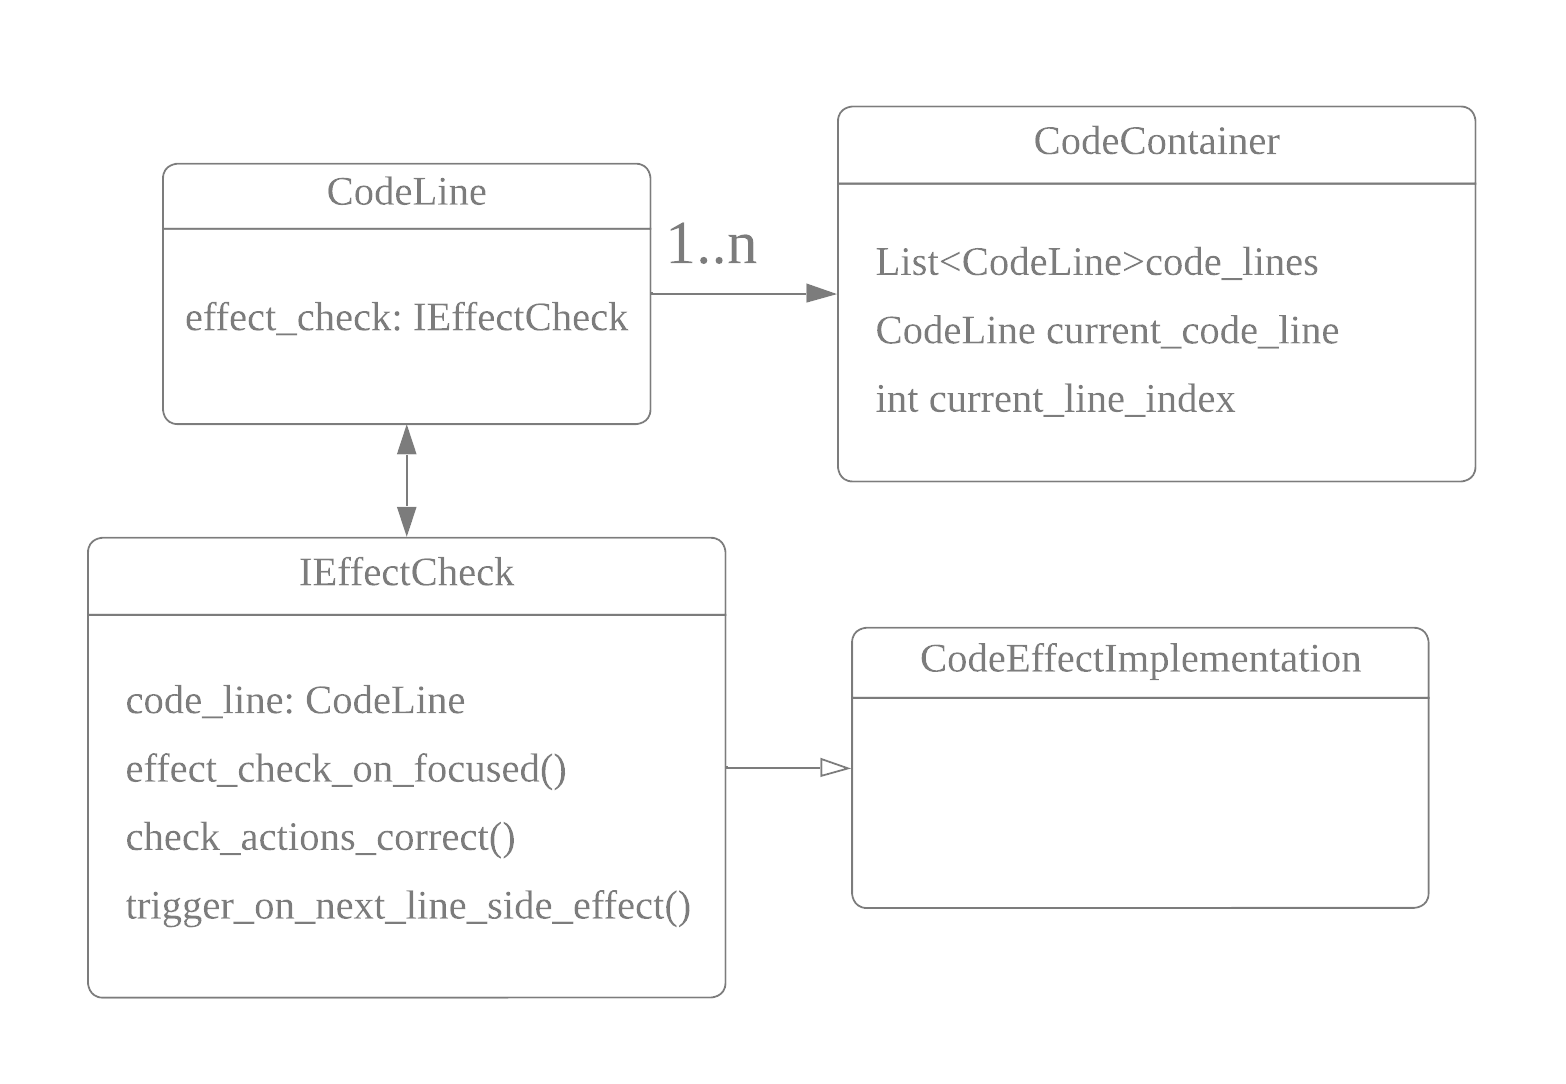
\includegraphics[width=0.9\textwidth]{imagenes/ArquitecturaSoftwareClasesNiveles.png}
	\caption{Arquitectura de software encargada de la mecánica de ejecución de código dentro del juego.}
	\label{CodeLinesArchitecture}
\end{figure}

Durante el juego, respecto a cómo avanzar en el código, el usuario debe ejecutar las acciones requeridas por el código correctamente. Si estas son correctas, el usuario pasa a la siguiente instrucción, desbloqueando nuevas tareas.

La acción que debe ejecutar el usuario está contenida entre las funciones effect\_check\_on\_focused() y check\_actions\_correct() (Tabla \ref{table_effect_check_methods}). Estas dependerán de cada línea de código. Por ejemplo, en la figura (\ref{InterfazBFS} ) que muestra el código de BFS, la primera línea dice t = starting\_node. En este caso, el jugador debe hacer click en el nodo 0.

La clase CodeLine contiene la lógica de una única línea de código. Entre sus funciones se encuentran: dar énfasis visual a la línea de código actual, proporcionar feedback audiovisual al usuario cuando la instrucción de la línea se completa correctamente y verificar constantemente si la instrucción de línea se ha completado correctamente (ver figura \ref{CodeLinesArchitecture}).


Cada CodeLine tiene asociado un script que puede ser especificado desde el editor de Godot a través de una variable exportada. Este script debe heredar de la clase EffectCheck, la cual actúa como interfaz. Cada script que implemente la interfaz EffectCheck debe definir métodos para: 1) cuando el puntero de instrucción llega a la línea del script; 2) verificar que la instrucción actual se ha realizado correctamente; y 3) si es necesario, manejar efectos colaterales de la instrucción. Este último se utiliza en los ciclos for, donde se mueve el índice utilizado para avanzar por los ciclos y recorrer arreglos, así como para la creación de variables.

En el panel inferior, se encuentran dos clases esenciales: DebugBlock y ADTShower. DebugBlock se encarga de mostrar las variables instanciadas, su nombre y su valor actual. Contiene la lógica para agregar, modificar o eliminar alguna variable. Cada vez que se pasa por un ciclo for o se declara una variable, este ajusta sus variables internas. Hay una variable seleccionada que puede ser manipulada por el usuario de diversas maneras. Al presionar la flecha hacia arriba, se selecciona la variable que está encima de la actual y viceversa para la flecha hacia abajo. En la figura \ref{BFSFullGame}, se observa que la variable ``q'' está seleccionada.

\begin{figure}[h]
	\centering
	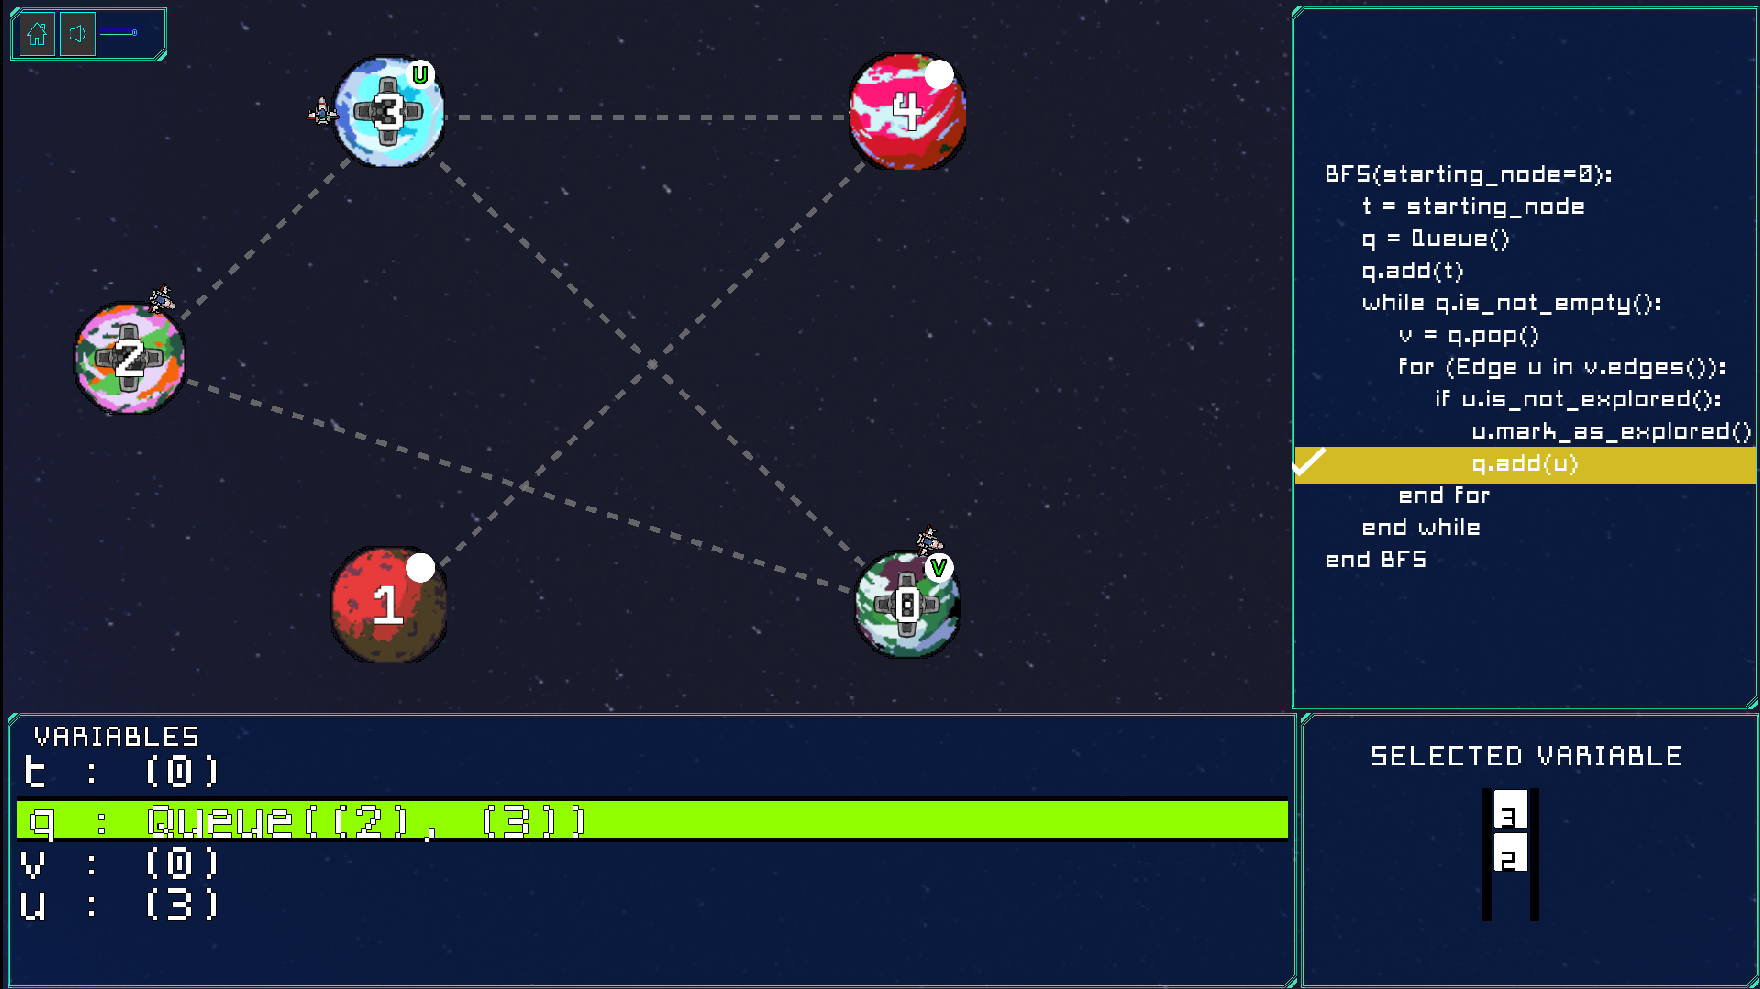
\includegraphics[width=0.9\textwidth]{imagenes/BFSFullGame.png}
	\caption{Nivel jugable BFS. Se observa el código a la derecha, el grafo en el centro, el DebugBlock en la parte inferior izquierda y el ADTShower en la esquina inferior derecha. La varible q está seleccionada.}
	\label{BFSFullGame}
\end{figure}

La clase ADTShower se encarga de mostrar en la esquina inferior derecha la variable que ha sido seleccionada por el usuario. Esta visualiza al objeto, enfatizando cuando un nodo se agrega o elimina de una cola o pila, lo cual depende del algoritmo que se esté enseñando, BFS o DFS, respectivamente.

Inicialmente, cada vez que se creaba un nuevo script por una nueva línea de código se debían modificar las clases DebugBlock, ADTShower y StoredData (explicada más adelante). Además, estos efectos debían reflejarse en las líneas de código siguientes para lograr cohesión. Por ejemplo, si la quinta línea crea la variable ``u'' y la sexta la modifica, esto se debe reflejar correctamente en todas las estructuras mencionadas.

Para resolver el problema del alto costo de implementación, se optó por crear una clase llamada ADTMediator, siguiendo el patrón Mediator \cite{Freeman2015TheMP}. Esta clase se inspiró en la arquitectura de React, donde el código generado por React funciona como una ``única fuente de verdad'' o ``Single Source of Truth'' \cite{ReactSingleSourceOfTruth}. Con esta arquitectura, se envía un mensaje a ADTMediator para solicitar la modificación, creación o eliminación de una variable. Posteriormente, esta clase ajusta sus variables internas y luego notifica a las clases DebugBlock y ADTShower qué información mostrar.

Una desventaja de esta arquitectura es que realiza copias innecesarias en cada paso, perdiendo eficiencia. Sin embargo, dado que se trabaja con menos de seis variables, este costo es despreciable a nivel de usuario.

\begin{figure}[h!]
	\centering
	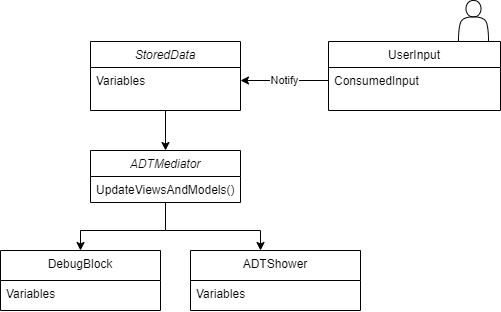
\includegraphics[width=0.9\textwidth]{imagenes/ArquitecturaMediatorAfter.png}
	\caption{Diagrama de un nivel utilizando el ADTMediator, reduciendo el acoplamiento entre clases.}
	\label{ArquitecturaMediatorAfter}
\end{figure}

Una clase que sirve de puente para comunicarse con el ADTMediator es StoredData. Este es un singleton que contiene datos, tales como los avances del usuario en los distintos niveles y el estado del juego. Cuando una línea de código busca modificar variables dentro del juego, ejecuta un método de este singleton, el cual reenvía esta información al ADTMediator. Se optó por esta metodología, pues es fácil obtener el puntero a StoredData, ya que usa el patrón singleton.

Otros singletons son: AudioPlayer, encargado de emitir sonidos específicos en cualquier momento del juego, y NotificationManager, que genera ventanas emergentes para el usuario, como menús, avisos o pestañas donde se debe responder sí o no.

\subsection{Cómo agregar una nueva CodeLine y ajustarse a otro algoritmo}

El framework creado en IGACSE permite la creación de líneas nuevas de código en menos de diez pasos. Facilitando la reproducción de algoritmos de manera precisa. En este capítulo se entrega un ejemplo y muestras de código. En primer lugar, se debe crear el script que ejecuta una línea de código en el programa. Para esto, se debe crear un nuevo archivo GDScript que herede de la clase EffectCheck como se muestra en la figura \ref{effect_check_script}.

\begin{figure}[h!]
	\centering
	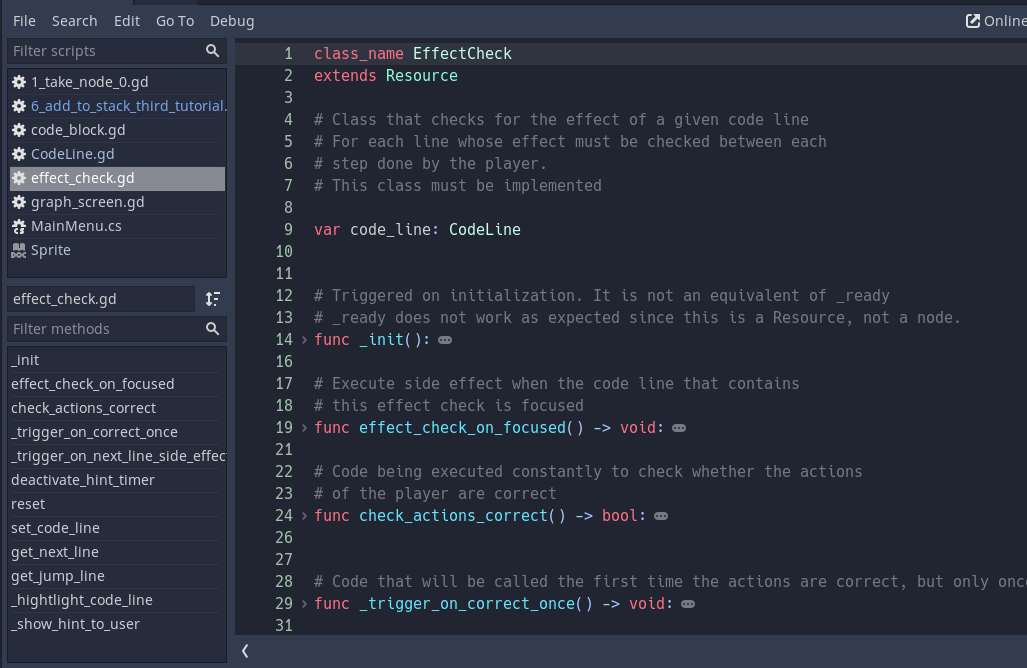
\includegraphics[width=0.9\textwidth]{imagenes/effect_check_script.png}
	\caption{Script de la clase abstracta EffectCheck.}
	\label{effect_check_script}
\end{figure}

Los métodos de esta clase que pueden ser redefinidos según cada caso. Estos se pueden ver en la tabla \ref{table_effect_check_methods}. 

\newgeometry{margin=0.5in}

\begin{table}[h]
    \centering
    \begin{tabular}{|l|p{0.6\textwidth}|}
        \hline
        \textbf{Método} & \textbf{Acción} \\
        \hline
        effect\_check\_on\_focused & Cuando el puntero de instrucciones alcanza esta línea de código, esta función ejecuta un efecto dependiendo del caso, por ejemplo, permitir que un nodo sea seleccionable.\\
        \hline
        check\_actions\_correct & Verifica constantemente si el jugador ha actuado acorde a la instrucción. Retorna verdadero si el usuario ha completado las acciones relacionadas con esta línea de código.  \\
        \hline
        \_trigger\_on\_correct\_once & Acción que ejecuta la función cuando la instrucción se ha completado correctamente. Se ejecuta a lo más una vez. Por ejemplo, al presionar un planeta correctamente, deseamos visualizar una nave espacial volando hacia dicho planeta \\
        \hline
		\_show\_hint\_to\_user & Qué se muestra cuando el usuario tarda cierto tiempo en ejecutar correctamente las acciones requeridas por la instrucción, como mostrar un ratón haciendo click en un planeta. Cumple el objetivo de ayudar al jugador a avanzar. \\
        \hline
        \_trigger\_on\_next\_line\_side\_effect & Acción que ejecuta la función cuando se llega a la siguiente línea. De manera predeterminada, es apagar el timer para entregar un hint.\\
        \hline
        reset & Acción llevada a cabo cuando se llega la siguiente instrucción. Utilizado en ciclos y condicionales para asegurarse de que cuando se vuelvan a repetir tales instrucciones, la ejecución funcione como se espera.  \\
        \hline
        get\_next\_line & Retorna el índice al que debería avanzar el puntero de instrucciones al terminar la función, si es que no corresponde un salto. \\
        \hline
        get\_jump\_line & Retorna el índice al que debería saltar el puntero de instrucciones al terminar la función. Utilizada en condicionales y ciclos. Esta función se diferencia de la anterior porque permite saltar líneas. \\
        \hline
    \end{tabular}
    \caption{Descripción de los métodos que pueden ser redefinidos por las implementaciones de la clase abstracta EffectCheck.}
    \label{table_effect_check_methods}
\end{table}

\restoregeometry

A modo de ejemplo, en la figura \ref{v_is_not_explored_effect_check} se muestra la instrucción \emph{If v.is\_not\_explored()} usada en el algoritmo DFS. Esta instrucción asegura que un mismo nodo no sea explorado más de una vez. Se le pregunta al usuario si se ha explorado el nodo v. Una vez el usuario ha contestado correctamente, se le permite avanzar.

\begin{figure}[h!]
	\centering
	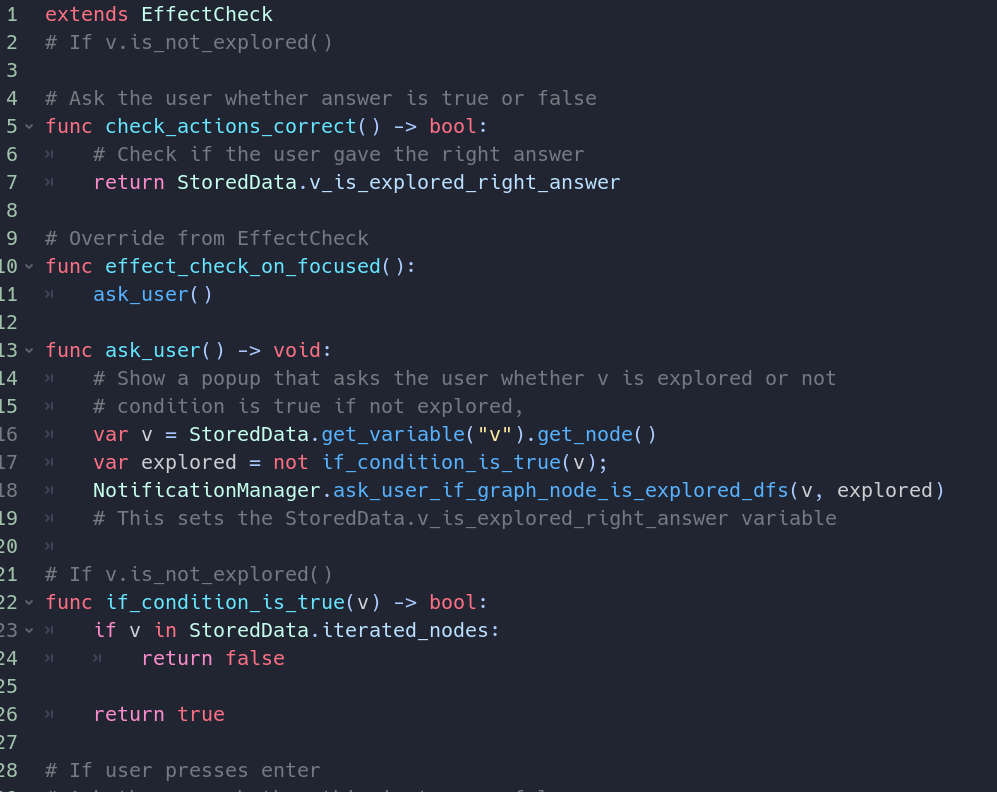
\includegraphics[width=0.9\textwidth]{imagenes/v_is_not_explored_effect_check_1.png}
	\caption{Script de la instrucción \emph{If v.is\_not\_explored()}.}
	\label{v_is_not_explored_effect_check}
\end{figure}

Para crear una nueva línea perteneciente a un algoritmo, es necesario generar un nuevo objeto que herede de CodeLine. Posteriormente, se deben redefinir los métodos de esta clase según el comportamiento esperado. 

Por ejemplo, en el caso de \emph{If v.is\_not\_explored()}, es esperable que al usuario se le pregunte si el nodo v está explorado una vez que se alcanza esta parte del código (Ver función effect\_check\_on\_focused en la figura \ref{v_is_not_explored_effect_check}). La instrucción se finaliza cuando el usuario responde correctamente si el nodo v ha sido explorado o no (Líneas 5 a 7 en la figura \ref{v_is_not_explored_effect_check}).

Respecto a la implementación de una nueva línea de código a nivel de usuario, el proceso es como se indica en la figura \ref{Godot_v_is_not_explored}. 

\begin{figure}[!h]
	\centering
	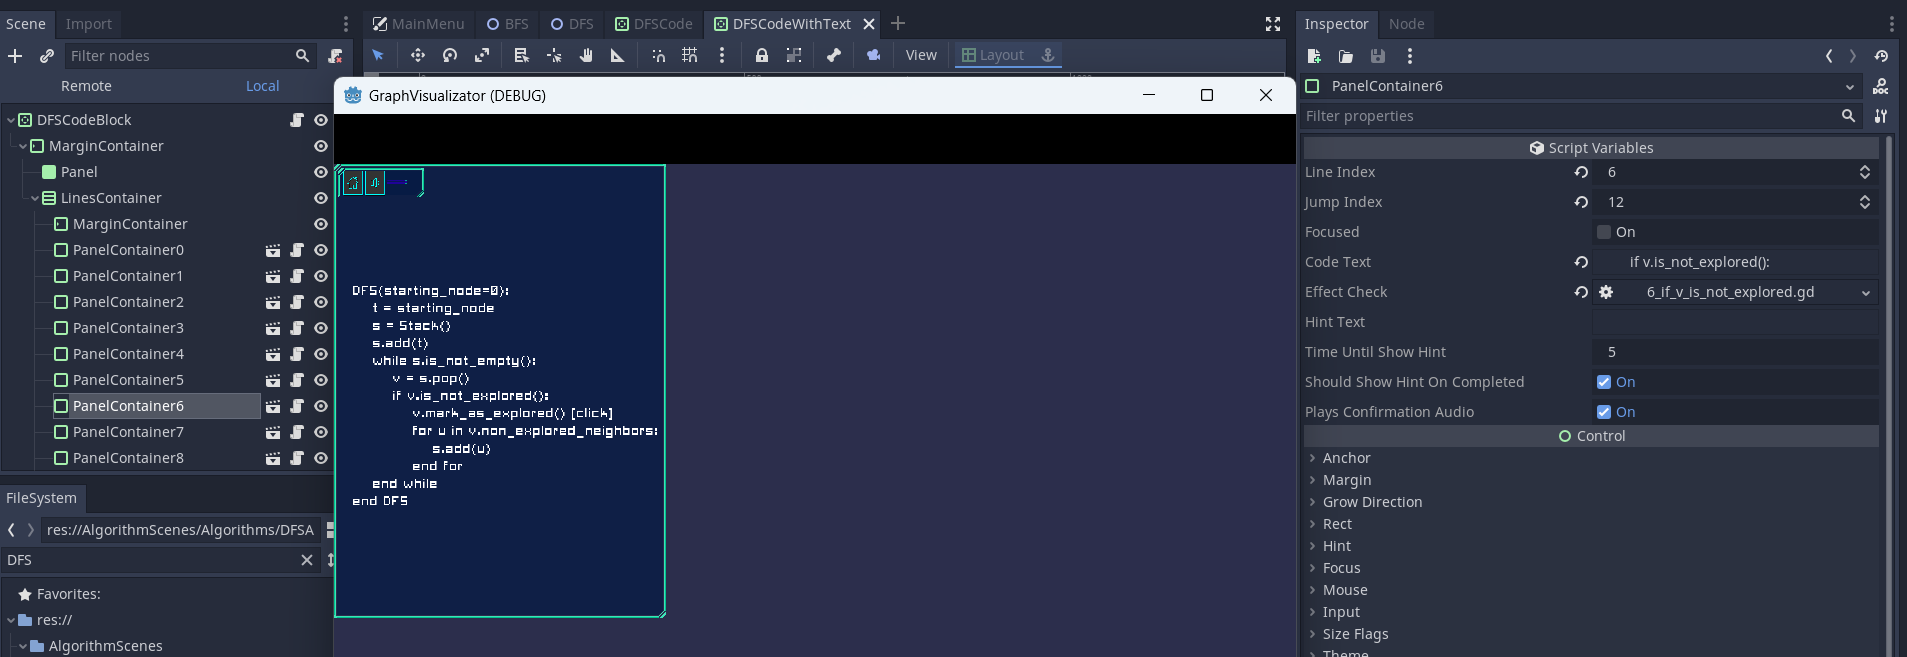
\includegraphics[width=0.8\textwidth]{imagenes/DFS_if_v_is_not_explored.png}
	\caption{Ventana de Godot mostrando un nodo que contiene la instrucción \emph{If v.is\_not\_explored()}.}
	\label{Godot_v_is_not_explored}
\end{figure}

Se debe tener un CodeBlock como raíz de un árbol jerárquico. Este CodeBlock debe contener un nodo del tipo VBoxContainer que se encarga de alinear los elementos de forma vertical. Dentro de este VBoxContainer, denominado LinesContainer en este caso, se encuentran los PanelContainers que, en realidad, representan las CodeLines (Ver figuras \ref{Godot_v_is_not_explored}).

Cada CodeLine tiene ciertas variables exportadas, como se observa en el lado derecho de la figura \ref{Godot_v_is_not_explored}. Estas variables se pueden ver en la tabla \ref{table_code_line_variables}

\begin{table}[!h]
    \centering
    \begin{tabular}{|l|p{0.8\textwidth}|}
        \hline
        \textbf{Variable} & \textbf{Descripción} \\
        \hline
        line\_index & Número de línea que representa la CodeLine. Sirve para indicar la siguiente línea, o a cuál línea saltar. \\
        \hline
        jump\_index  & Línea a la cual saltar en caso de que corresponda un salto. Utilizada en casos de condicionales y bucles. \\
        \hline
        focused & Su valor es verdadero cuando la línea de código está seleccionada. \\
        \hline
		code\_text & El texto del código que se muestra en pantalla. \\
        \hline
        effect\_check & Una referencia al script que hereda de EffectCheck y que determina la lógica de lo que hace la línea de código. \\
        \hline
        hint\_text  & El texto que se le mostrará al usuario si se demora en realizar alguna acción y está atascado. \\
        \hline
        time\_until\_show\_hint & Tiempo que transcurre desde que el puntero de instrucciones apunta a la instrucción y que se muestra el hint. \\
        \hline
    \end{tabular}
    \caption{Descripción de las variables exportadas de la clase CodeLine.}
    \label{table_code_line_variables}
\end{table}


Cada efecto desencadena modificaciones en las estructuras de datos del nivel. Por ejemplo, al crear la variable \emph{v} al recorrer un grafo, StoredData guarda una referencia a esta nueva variable, el ADTMediator es notificado y reenvía esta señal a las clases DebugBlock y ADTShower, permitiéndoles desplegar este objeto como un elemento visible en el juego.



\subsection{Arquitectura de software de un nivel de IGACSE}

% Contar que por sobre todo están los singletons y el GraphManager que se encarga de inicializar el grafo y el nivel.
% El GraphManager tiene una refernecia al ADT Mediator y al StoryBeforeLevel, que se encarga de mostrar la historia y dar una introducción a la teoría del nivel. Además, referencias a las popups.
% Dentro de la pantalla o Screen, están: DebugBlock, ADTShower y NodeContainer.
% Dentro del NodeContainer aparece cada nodo y las uniones de los arcos entre ellos.

Un nivel en IGACSE está compuesto por varios nodos de Godot. Los nodos más relevantes y específicos para esta aplicación se detallan en la figura \ref{diagram_dfs_level}, que muestra un ejemplo del nivel utilizando el algoritmo DFS.

\newgeometry{margin=0.5in}

\begin{figure}[!h]
	\centering
	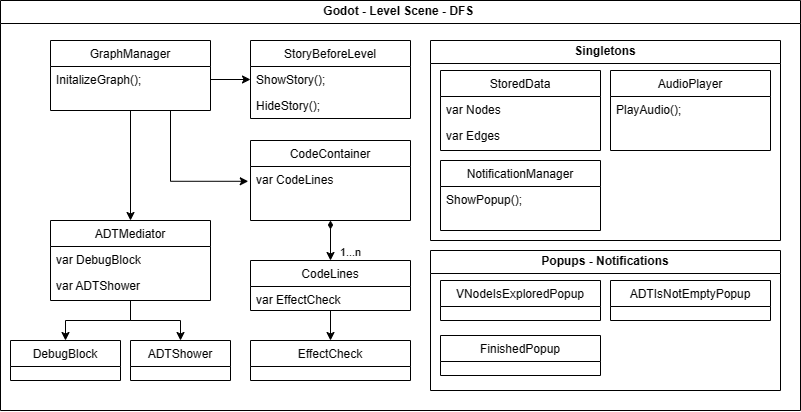
\includegraphics[scale=.7]{imagenes/level_scene_DFS.png}
	\caption{Diagrama simplificado de clases e interacciones del nivel DFS. Algunas clases y objetos no están agregados por motivos de simplicidad.}
	\label{diagram_dfs_level}
\end{figure}

\restoregeometry

En este caso, los singletons son aquellas clases que se mantienen durante todo el juego. AudioPlayer administra los sonidos y música de fondo del videojuego, mientras que NotificationManager maneja las popups que se cierran y abren durante el juego, relacionadas con menús y preguntas del tipo if.

En cuanto al singleton StoredData, este almacena información sobre los niveles jugados, las acciones realizadas por el jugador, el estado de avance y las variables en juego actualmente. Además, esta clase proporciona una librería de funciones relacionadas con la manipulación de variables durante el nivel, como funciones para obtener los datos relacionados a una variable a partir de un nombre en forma de texto.

La clase GraphManager inicializa el grafo y proporciona las referencias de nodos y arcos a StoredData. También indica a StoryBeforeLevel que debe mostrar un diálogo específico antes de comenzar el nivel jugable.

Posteriormente, se inicializan el ADTMediator, DebugBlock y ADTShower, cuyos roles ya fueron explicados anteriormente. En conjunto con estos objetos, el CodeContainer aparece en el nivel, construyendo cada línea de código con sus respectivos scripts.

El jugador introduce inputs, lo que le permite avanzar a lo largo de las líneas de código hasta completarlas todas. Una vez finalizado el algoritmo, StoredData se encarga de realizar la transición al siguiente nivel.

